\documentclass[lettersize,journal]{IEEEtran}
\usepackage[utf8]{inputenc}
\usepackage{graphicx}
\usepackage{hyperref}
\usepackage{xcolor}
\usepackage{comment}
\usepackage{minted}
\usepackage{amsmath,amssymb,amsthm}
\usepackage{caption}
\usepackage{array}
\usepackage{tabularray}
\usepackage{geometry}
\usepackage{textcomp}
\usepackage{stfloats}
\usepackage{url}
\usepackage{tabularx}
\usepackage{booktabs}
\usepackage{multirow}
\usepackage{wrapfig}
\usepackage{subcaption}
\usepackage[font=small,skip=4pt]{caption}
\geometry{verbose,tmargin=1in,bmargin=1in,lmargin=1in,rmargin=1in}

\newtheorem{definition}{Definition}
\newtheorem{insight}{Insight}
\newcommand{\ignore}[1]{}

\begin{document}

\title{Affective Susceptibility of Investors: A Pilot Study of Stock Return Co-Movement with Emotional Media Content}

\author{%
  \IEEEauthorblockN{%
    Bonnie Rushing\IEEEauthorrefmark{1}\IEEEauthorrefmark{2},
    William Hersch\IEEEauthorrefmark{1},
    and
    Shouhuai Xu\IEEEauthorrefmark{2}\\
  }%
  \IEEEauthorblockA{\IEEEauthorrefmark{1}US Air Force Academy }%
  \IEEEauthorblockA{\IEEEauthorrefmark{2}University of Colorado Colorado Springs }%
}

\maketitle

\begin{abstract}
We investigate whether aggregated media sentiment exhibits directional influence consistent with short-horizon stock return variation in a financial decision environment. Using 15{,}900+ media articles across fourteen U.S. equities spanning seven sectors---technology, semiconductors, automotive, finance, healthcare, energy, consumer staples, industrials, and media---over the period October 2024 to May 2025, we compute daily sentiment using VADER and examine its relationship with daily log returns. To move beyond contemporaneous correlation, we incorporate three complementary analyses: same-day association, lagged sentiment-to-return tests, and market-controlled regressions using SPY as a broad-market proxy. We additionally examine whether extreme sentiment realizations are followed by distinguishable next-day return behavior. The fourteen case studies reveal heterogeneous patterns that vary systematically across sectors: semiconductor stocks (Nvidia, AMD) and select media-entertainment firms (Disney) exhibit the strongest positive sentiment--return association, while non-technology sectors (healthcare, energy, consumer staples) exhibit near-zero or negative association. Tesla continues to exhibit near-zero association despite high media volume. Notably, extreme-sentiment events produce statistically significant next-day return effects for Microsoft ($p < 0.001$) and AMD ($p = 0.025$). We interpret these findings through a behavioral lens that includes investor attention, media saturation, sector-specific information environments, and noise discounting. Although the study does not claim definitive causal identification, it provides cross-sector directional evidence consistent with sentiment-linked return effects under controlled conditions.
\end{abstract}

\begin{IEEEkeywords}
affective computing, investor sentiment, media sentiment, stock returns, behavioral finance, financial text analysis, cognitive security, cross-sector analysis
\end{IEEEkeywords}

\textit{The views expressed in this article are those of the authors and do not necessarily reflect the official policy or position of the Air Force, the Department of Defense, or the U.S. Government.}

\section{Introduction}
\nocite{*}

Financial markets respond not only to firm fundamentals and macroeconomic conditions, but also to the information environment in which investors operate \cite{campbell1997econometrics}. 
News headlines, opinion pieces, and other digitally distributed narratives can shape expectations, amplify investor attention, and contribute to short-horizon trading behavior \cite{tetlock2007giving, LI2014826, CHANG2025101045}. 
Prior research demonstrates that media tone and public sentiment extracted from textual data can influence investor perceptions and market activity, particularly when information spreads rapidly through digital platforms \cite{bollen2011twitter, zhang2020stock}. 
This broader informational environment is relevant to affective computing because emotionally charged content may alter perception, judgment, and action in settings where human decisions are increasingly mediated by algorithmic platforms, recommender systems, and real-time data feeds \cite{hutto2014vader}.

A large literature has examined the relationship between textual sentiment and market behavior, including work on media tone, investor mood, and stock prediction \cite{tetlock2007giving, bollen2011twitter, zhang2020stock, LI2014826}. 
These studies collectively demonstrate that sentiment signals extracted from news articles, social media, or other digital text streams may correlate with financial market dynamics \cite{CHANG2025101045}. 
However, many existing studies focus on predictive modeling or forecasting performance rather than descriptive analysis of sentiment–return relationships at the individual equity level. 
Consequently, fewer studies examine a narrower question that is particularly relevant to affective computing and behavioral finance: when sentiment is aggregated at the daily level for a specific stock, how much short-horizon co-movement appears between that stock's media sentiment and its daily return, and how does that observed association vary across equities?

This paper addresses that question through a multi-sector empirical study. Specifically, we analyze 15{,}900+ articles linked to fourteen U.S. equities across seven sectors---including technology (Apple, Alphabet, Amazon, Microsoft, Meta), semiconductors (Nvidia, AMD), automotive (Tesla), finance (JPMorgan), healthcare (Johnson \& Johnson), energy (ExxonMobil), consumer staples (Walmart), industrials (Boeing), and media (Disney)---over the period October 2024 to May 2025. We aggregate article-level VADER sentiment into daily stock-level sentiment signals, align those signals to trading days, and compare them with daily log returns. We then estimate descriptive sentiment--return association using Pearson correlation and a simple market-adjusted variant that removes same-day broad market movement using the S\&P 500 ETF (SPY) \cite{sp500index} as a proxy.

The contribution of this paper is not a claim of definitive causal identification. Rather, we test whether media sentiment exhibits directional structure consistent with short-horizon return effects under constrained empirical conditions. To do so, we complement contemporaneous sentiment--return association with lagged analyses, market-controlled regression models, and an event-based examination of extreme sentiment realizations. This framing enables a more rigorous assessment than simple same-day correlation while remaining appropriately cautious given the limits of the available data.

The case studies suggest heterogeneous patterns that vary systematically across sectors. Semiconductor stocks (Nvidia, AMD) and select entertainment firms (Disney) exhibit the strongest positive sentiment--return association. Technology firms show moderate but variable association. Non-technology sectors---finance, healthcare, energy, consumer staples---generally exhibit weak or near-zero association, suggesting that sentiment-linked return effects may be concentrated in sectors with high retail investor participation and narrative-driven valuation. Tesla, despite the highest media volume in the sample, continues to exhibit near-zero association, consistent with saturation and noise-discounting interpretations. Notably, extreme-sentiment event analysis reveals statistically significant next-day return effects for Microsoft and AMD, providing the strongest directional evidence in the study. We interpret this heterogeneity through the lenses of sector-specific information environments, investor composition, attention allocation, and media saturation.

\subsection{Contributions}
This paper makes five contributions.

First, it presents a reproducible pipeline for constructing stock-level daily sentiment measures from article-level financial news data, including explicit discussion of ticker selection, date filtering, aggregation, and trading-day alignment.

Second, it extends the analysis from a five-stock technology-focused sample to a fourteen-stock, seven-sector cross-sectional design, enabling direct comparison of sentiment--return relationships across fundamentally different market segments.

Third, it evaluates whether sentiment exhibits directional influence consistent with short-horizon stock return behavior by combining contemporaneous association, lagged sentiment-to-return tests, and market-controlled regression analysis.

Fourth, it examines whether extreme sentiment realizations are followed by distinguishable next-day return behavior, providing an event-based perspective on sentiment-linked market response---and identifies two equities (Microsoft and AMD) where these effects are statistically significant.

Fifth, it interprets heterogeneous cross-sector results through a behavioral framework grounded in attention, investor composition, sector-specific information environments, and noise discounting, while clearly identifying the limits of inference.

\subsection{Scope of Inference}
This study does not claim definitive causal identification in the strong econometric sense, nor does it rule out all omitted-variable bias. However, it \textit{does} assess whether media sentiment exhibits directional and statistically structured relationships with subsequent stock returns after partial control for market-wide movement. The results, therefore, should be interpreted as evidence consistent with sentiment-linked return effects under controlled conditions, rather than as purely contemporaneous descriptive co-movement. The study also does not support broad claims about all equities, all investors, or long-run dynamics, and it should not be read as validating a deployable trading strategy.

\subsection{Paper Outline}
Section \ref{sec:related} reviews related work. Section \ref{sec:preliminaries} introduces the behavioral framing used to interpret the results. Section \ref{sec:data_method} presents the data pipeline and methodology. Section \ref{sec:results} reports the case-study results. Section \ref{sec:discussion} discusses interpretation, anomaly detection, and implications. Section \ref{sec:limitations} describes limitations. Section \ref{sec:conclusion} concludes.

\section{Related Work}
\label{sec:related}
Research connecting textual sentiment and financial markets spans several literatures.

One body of work studies how media tone and textual features relate to returns, volatility, and investor attention. Tetlock's classic study showed that media pessimism is associated with market outcomes \cite{tetlock2007giving}. Loughran and McDonald demonstrated that general-purpose sentiment dictionaries can perform poorly in financial contexts and motivated more careful text analysis in finance \cite{loughran2011liability}. Other work has studied sentiment from social media and online discussion, including evidence that aggregated mood signals may contain predictive information under some conditions \cite{bollen2011twitter,zhang2020stock}.

A second body of work in behavioral finance explains why emotionally salient or highly available information may shape decisions, especially when investors rely on heuristics rather than deliberate valuation. Kahneman's dual-system account provides a useful conceptual lens here \cite{kahneman2011thinking}. Related scholarship on investor sentiment, attention, and limits to arbitrage helps explain why narrative intensity may matter more in some settings than others.

A third body of work concerns financial manipulation, information operations, and cyber-enabled market disruption. Research on the economic effects of publicly announced breaches \cite{10.5555/876661.876669} and on broader cognitive-security concerns suggests that information environments can have economically meaningful consequences. More recent work has also raised concern about generative AI, deepfakes, and fabricated financial narratives as tools for manipulating investor perception \cite{shamo2024deepfake}.

This paper differs from prior work in three ways. First, it focuses on a transparent stock-level pilot pipeline rather than a large-scale prediction benchmark. Second, it emphasizes descriptive co-movement rather than causal claims. Third, it bridges financial text analysis and affective computing by asking how emotionally coded media environments may align with short-horizon investor-facing outcomes, while being explicit about the limits of inference.

\section{Preliminaries}
\label{sec:preliminaries}

\subsection{Dual-System Cognition as an Interpretive Lens}
\begin{definition}[System 1 Thinking \cite{kahneman2011thinking}]
System 1 thinking is fast, automatic, intuitive, and heuristic-driven. It relies on associative processing and often produces quick judgments with limited deliberation.
\end{definition}

\begin{definition}[System 2 Thinking \cite{kahneman2011thinking}]
System 2 thinking is slower, effortful, reflective, and analytical. It is engaged when individuals evaluate evidence, override intuition, and reason more deliberately.
\end{definition}

We use dual-system cognition as an interpretive framework rather than as a tested causal model in this paper. In fast-moving financial contexts, emotionally salient headlines may preferentially engage System 1 responses, especially among attention-constrained or less experienced investors \cite{kahneman2011thinking, barber2008all}. By contrast, investors who rely more heavily on valuation models, portfolio constraints, or institutionally mediated decision processes may be less reactive to the emotional surface of news content \cite{campbell1997econometrics}. This framing provides a language for discussing why some equities may exhibit stronger short-horizon sentiment association than others.

\subsection{Investor Attention, Noise, and Saturation}

A high volume of media coverage does not necessarily imply a strong sentiment--return relationship. Under some conditions, heavy repeated coverage may reduce the marginal informativeness of any single item. Investors may discount repetitive narratives as noise, especially when coverage is sensationalized, polarized, or weakly linked to fundamentals \cite{tetlock2007giving, barber2008all, LI2014826}. This phenomenon aligns with the broader literature on limited investor attention and noise trading, which suggests that investors process only a subset of available information and may treat excessive media signals as background noise rather than actionable information \cite{bollen2011twitter, CHANG2025101045}. This leads to our synthesized definition of \textit{noise discounting}.

\begin{definition}[Noise Discounting]
Noise discounting is the tendency of investors to down-weight or ignore information perceived as repetitive, low credibility, weakly diagnostic, or excessively sensational relative to firm fundamentals.
\end{definition}

Noise discounting behavior is consistent with the literature on noise trading and limited investor attention, where market participants selectively filter large volumes of information and treat some signals as informational noise rather than actionable news \cite{black1986noise, barber2008all, tetlock2007giving}.

This concept is useful for interpreting cases such as Tesla in our sample, where media volume is unusually high but descriptive sentiment association is near zero.

\subsection{Subjective and Objective Drivers of Investor Response}

Investor reactions are shaped by both objective and subjective factors. Objective factors include earnings announcements, forward guidance, macroeconomic conditions, regulation, and sector-wide shocks that affect firm fundamentals and expected cash flows \cite{campbell1997econometrics}. Subjective factors include prior beliefs, identity, digital culture, emotionality, social-group affiliation, and trust in information sources, which may influence how investors interpret and respond to information signals \cite{bollen2011twitter, LI2014826, CHANG2025101045}. 

We do not directly measure these individual-level factors in this paper. However, acknowledging them is essential because they limit what can be inferred from aggregate sentiment measures. Stock-level media sentiment is therefore best understood as one observable signal within a broader socio-technical decision environment in which human judgment, digital information systems, and behavioral biases jointly influence market outcomes \cite{tetlock2007giving, kahneman2011thinking}.

\subsection{Interpretation of Sentiment--Return Association}
It is important to distinguish between contemporaneous co-movement, directional structure, and definitive causal identification. Same-day correlation between aggregated media sentiment and stock returns measures statistical association, but by itself does not establish directional influence. Stock prices are simultaneously affected by macroeconomic trends, sector-wide shocks, firm-specific information, and broader market sentiment \cite{campbell1997econometrics}.

For this reason, the present study does not rely solely on contemporaneous correlation. Instead, it incorporates lagged sentiment-to-return tests, market-controlled regression analysis, and event-based examination of extreme sentiment realizations. These additional analyses do not eliminate all confounding, but they provide a stronger basis for assessing whether sentiment exhibits directional influence consistent with causal mechanisms. Accordingly, we interpret the findings as controlled directional evidence rather than as purely descriptive co-movement.

\section{Data and Methodology}
\label{sec:data_method}

\subsection{Research Questions}
The study addresses four research questions:
\begin{itemize}
    \item \textbf{RQ1}: How should daily stock-level media sentiment be quantified from article-level text?
    \item \textbf{RQ2}: To what extent is aggregated media sentiment associated with short-horizon daily log returns in the selected equities?
    \item \textbf{RQ3}: Does lagged sentiment exhibit directional structure with subsequent returns after partial control for market-wide movement?
    \item \textbf{RQ4}: What behavioral mechanisms may help explain heterogeneity in observed sentiment--return relationships across the five case studies?
\end{itemize}

\subsection{Data Sources and Collection Pipeline}
The data pipeline was derived from project files inspired by FinAgent \cite{zhang2024finagent}. Daily closing prices were retrieved from the Financial Modeling Prep (FMP) stable API\footnote{https://site.financialmodelingprep.com/}, while company-linked news articles were collected from the Finnhub API\footnote{https://finnhub.io/}, which aggregates financial news from multiple publishers including Reuters, Benzinga, MarketWatch, and other major financial media outlets. To improve reproducibility, we specify the steps explicitly here.

\begin{enumerate}
    \item \textbf{Ticker universe selection.} We selected fourteen U.S. equities spanning seven sectors: technology (AAPL, GOOGL, AMZN, MSFT, META), semiconductors (NVDA, AMD), automotive (TSLA), finance (JPM), healthcare (JNJ), energy (XOM), consumer staples (WMT), industrials (BA), and media/entertainment (DIS). This cross-sector design enables comparison of sentiment--return relationships across fundamentally different market segments.
    \item \textbf{Date-window restriction.} We constrained retrieval to the study window from October 1, 2024 to May 31, 2025, providing approximately eight months of coverage.
    \item \textbf{Price retrieval.} For each ticker and for the SPY market proxy, we collected daily closing-price series and converted them to daily log returns.
    \item \textbf{News retrieval.} We collected company-linked news items from Finnhub for each ticker within the specified window, using weekly chunked requests to maximize coverage. Duplicate articles were removed based on headline matching.
    \item \textbf{Sentiment scoring.} Each article headline and text summary was scored with VADER, producing negative, neutral, positive, and compound scores.
    \item \textbf{Daily aggregation.} Multiple article-level compound scores for a stock on a given day were aggregated into a single daily sentiment value using a 10\% trimmed mean.
    \item \textbf{Trading-day alignment.} Items published after 16:00 ET were aligned to the next market close to better match the decision environment facing investors.
\end{enumerate}

The resulting dataset includes 15{,}900+ sentiment-scored articles across the fourteen equities. The cross-sector design enables us to test whether sentiment--return relationships are concentrated in particular market segments or distributed broadly across equity types.


\subsection{Sentiment Quantification}

We use VADER \cite{hutto2014vader}, a lexicon- and rule-based sentiment analyzer designed for short informal text. Lexicon-based sentiment methods have been widely used in studies linking textual sentiment to financial market behavior \cite{tetlock2007giving, LI2014826}. VADER produces four scores: negative, neutral, positive, and compound. The compound score, ranging from $-1$ to $+1$, is the primary measure used in this study because it summarizes overall emotional polarity in a single continuous value.

Let $s_{j,t}$ denote the compound sentiment score for article $j$ associated with stock $k$ on date $t$. Let $m_{k,t}$ denote the number of articles for stock $k$ on date $t$. We define the daily aggregated sentiment as a trimmed mean:
\begin{equation}
S_{k,t} = \operatorname{trimmean}\left(\{s_{j,t}\}_{j=1}^{m_{k,t}}, 10\%\right).
\end{equation}
We use a trimmed mean to reduce the influence of extreme article-level scores.

VADER is attractive in this setting because it is transparent, computationally lightweight, and widely used in sentiment analysis research. At the same time, it has well-known limitations: it may miss sarcasm, domain-specific framing, and subtleties of financial discourse. We therefore treat the resulting sentiment values as approximate affective indicators rather than ground truth.

\subsection{Return Construction}

To reduce spurious association that can arise from price levels, we analyze daily log returns rather than raw closing prices, a standard practice in financial econometrics \cite{campbell1997econometrics}. Let $P_{k,t}$ be the closing price of stock $k$ on trading day $t$. The daily log return is
\begin{equation}
r_{k,t} = \ln\left(\frac{P_{k,t}}{P_{k,t-1}}\right).
\label{eq:log_return_main2}
\end{equation}


\subsection{Primary Descriptive Association Measure}
We estimate descriptive sentiment--return association using the Pearson correlation coefficient:
\begin{equation}
\rho_k = \frac{\sum_{t=1}^{n}(S_{k,t}-\bar{S}_k)(r_{k,t}-\bar{r}_k)}{
\sqrt{\sum_{t=1}^{n}(S_{k,t}-\bar{S}_k)^2}\sqrt{\sum_{t=1}^{n}(r_{k,t}-\bar{r}_k)^2}}.
\label{eq:pearson_main2}
\end{equation}

We use Pearson correlation because the goal is to summarize linear co-movement between two continuous daily variables over a short horizon \cite{howell2021statistical}. Importantly, we interpret $\rho_k$ as a descriptive statistic only. It does not identify direction, mechanism, or causal influence.

\subsection{Market-Adjusted Analysis}

To partially address confounding from broad market movement, we compute market-adjusted returns using SPY as a proxy for the overall U.S. equity market \cite{sp500index}. This adjustment is commonly used in financial studies to separate firm-specific movements from market-wide trends \cite{campbell1997econometrics}.
Let $r_{m,t}$ denote the daily log return of the SPDR S\&P 500 ETF (SPY), which we use as a proxy for market-wide movements \cite{sp500index}. We define the excess return:
\begin{equation}
r^{\mathrm{ex}}_{k,t} = r_{k,t} - r_{m,t}.
\label{eq:excess_main2}
\end{equation}
We then compute the descriptive association between $S_{k,t}$ and $r^{\mathrm{ex}}_{k,t}$. This does not solve the causal problem, but it helps determine whether the raw association is plausibly explained by market-wide drift alone.

\subsection{Lagged and Market-Controlled Directional Tests}
To assess whether sentiment exhibits directional structure beyond same-day co-movement, we estimate lagged association and controlled regression models.

First, we compute lagged correlations between daily sentiment and subsequent returns:
\begin{equation}
\rho^{(1)}_k = \mathrm{corr}(S_{k,t-1}, r_{k,t}),
\end{equation}
and, where sample length permits, a second lag:
\begin{equation}
\rho^{(2)}_k = \mathrm{corr}(S_{k,t-2}, r_{k,t}).
\end{equation}

Second, we estimate a market-controlled regression of the form
\begin{equation}
r_{k,t} = \alpha_k + \beta_k S_{k,t-1} + \gamma_k r_{m,t} + \varepsilon_{k,t},
\label{eq:controlled_reg}
\end{equation}
where $r_{m,t}$ is the daily log return of SPY. In this specification, $\beta_k$ captures whether lagged sentiment is associated with next-day stock returns after partial control for broad market movement.

These tests do not provide definitive causal identification. However, they improve inference in two important ways. First, the lag structure imposes temporal ordering, reducing concerns about same-day simultaneity. Second, the inclusion of market returns provides an explicit control for broad market drift. We therefore interpret significant positive or negative $\beta_k$ estimates as directional evidence consistent with sentiment-linked return effects under controlled conditions.

\subsection{Extreme-Sentiment Event Analysis}
We further assess directional structure using an event-based design centered on unusually large sentiment realizations. For each stock, we identify event days on which the absolute standardized sentiment score exceeds a threshold based on the stock's empirical distribution. Let
\begin{equation}
\tilde{S}_{k,t} = \frac{S_{k,t} - \mu_k}{\sigma_k},
\end{equation}
where $\mu_k$ and $\sigma_k$ are the sample mean and standard deviation of daily sentiment for stock $k$. We define an extreme-sentiment event as any day for which $|\tilde{S}_{k,t}| > \tau$, where $\tau$ is chosen to capture the upper tail of the sentiment distribution.

For these event days, we compare subsequent next-day returns $r_{k,t+1}$ with the baseline distribution of non-event next-day returns. This event-based analysis is intended to determine whether sentiment spikes are followed by distinguishable return behavior. While not a full causal event study in the classical finance sense, it provides an additional directional test that complements the lagged and controlled analyses.

\subsection{A Restrained Descriptive Typology}
To summarize the case-study results, we use a deliberately narrow typology of observed association. The typology is descriptive only.

\begin{definition}[Low Sentiment Association (LSA)]
A stock is in the LSA range when the observed sentiment--return correlation magnitude is small over the study window (e.g., $|\rho_k| < 0.30$). LSA indicates weak observed linkage in this sample and does not imply immunity to manipulation or irrelevance of sentiment under other conditions.
\end{definition}

\begin{definition}[Moderate Sentiment Association (MSA)]
A stock is in the MSA range when the observed sentiment--return correlation is positive and non-trivial over the study window (e.g., $0.30 \le \rho_k < 0.70$). MSA indicates moderate descriptive co-movement in this sample and does not establish causality.
\end{definition}

\subsection{Real-Time Sentiment Anomaly Detection: A Concrete Example}
One reviewer asked for a clearer explanation of what a real-time sentiment anomaly detection system would do. We therefore define a simple illustrative version here.

Suppose a rolling baseline of daily sentiment is maintained for stock $k$ over the previous $w$ trading days, with rolling mean $\mu_{k,t}^{(w)}$ and rolling standard deviation $\sigma_{k,t}^{(w)}$. A standardized sentiment anomaly score can be defined as
\begin{equation}
Z_{k,t} = \frac{S_{k,t} - \mu_{k,t}^{(w)}}{\sigma_{k,t}^{(w)}}.
\end{equation}
If $|Z_{k,t}| > 2$ and no corresponding firm filing, earnings release, guidance update, or other corroborating event is observed within the same window, the system could flag the day for analyst review. In practice, such a detector would not prove manipulation; it would simply identify unusual sentiment shifts whose informational basis is unclear. This idea follows the broader literature on statistical anomaly detection and financial market surveillance, where abnormal observations relative to historical baselines are flagged for further investigation rather than interpreted as causal evidence of manipulation \cite{howell2021statistical, chandola2009anomaly}. In this sense, we use the phrase ``sentiment anomaly detection system'' to describe a monitoring tool that highlights unusual sentiment movements for analyst review rather than an automated mechanism for identifying misconduct.

A summary of this methodology can be found at https://thebonnierushing.com/investor-susceptibility.

\section{Results}
\label{sec:results}

\subsection{Sample Overview}
The fourteen-stock dataset contains 15{,}900+ sentiment-scored media items over the study window. Table~\ref{tab:sample_overview} summarizes the article counts and average compound sentiment scores by sector.

\begin{table}[!htbp]
\centering
\caption{Sample Overview: Article Counts and Mean Sentiment by Ticker}
\label{tab:sample_overview}
\begin{tabular}{llrr}
\toprule
\textbf{Sector} & \textbf{Ticker} & \textbf{Articles} & \textbf{Mean $\bar{S}_k$} \\
\midrule
\multirow{5}{*}{Technology} & AAPL & 1{,}665 & 0.132 \\
 & GOOGL & 1{,}660 & 0.278 \\
 & AMZN & 1{,}638 & 0.347 \\
 & MSFT & 1{,}512 & 0.333 \\
 & META & 1{,}247 & 0.226 \\
\midrule
\multirow{2}{*}{Semiconductors} & NVDA & 1{,}857 & 0.246 \\
 & AMD & 826 & 0.363 \\
\midrule
Automotive & TSLA & 1{,}760 & 0.166 \\
\midrule
Finance & JPM & 752 & 0.181 \\
\midrule
Healthcare & JNJ & 457 & 0.264 \\
\midrule
Energy & XOM & 430 & 0.320 \\
\midrule
Consumer & WMT & 814 & 0.224 \\
\midrule
Industrials & BA & 875 & 0.181 \\
\midrule
Media & DIS & 458 & 0.296 \\
\bottomrule
\multicolumn{2}{l}{\textbf{Total}} & \textbf{15{,}951} & \\
\bottomrule
\end{tabular}
\end{table}

Several features of the sample are noteworthy. First, media coverage is substantially heavier for technology and semiconductor stocks than for non-technology sectors---Nvidia receives more than four times the coverage of Johnson \& Johnson. Second, mean sentiment is positive across all tickers, but varies from 0.132 (Apple) to 0.363 (AMD), suggesting that the emotional baseline of media coverage differs across firms. Third, Tesla's relatively low mean sentiment (0.166) combined with the second-highest article volume hints at the polarization dynamic discussed below.

\subsection{Case-Study Associations}

\subsubsection{Technology Sector}
Figure~\ref{fig:tech_stocks} shows normalized closing prices and normalized daily aggregated sentiment for the five technology equities.

\begin{figure*}[t!]
\centering
\begin{subfigure}[b]{0.47\textwidth}
    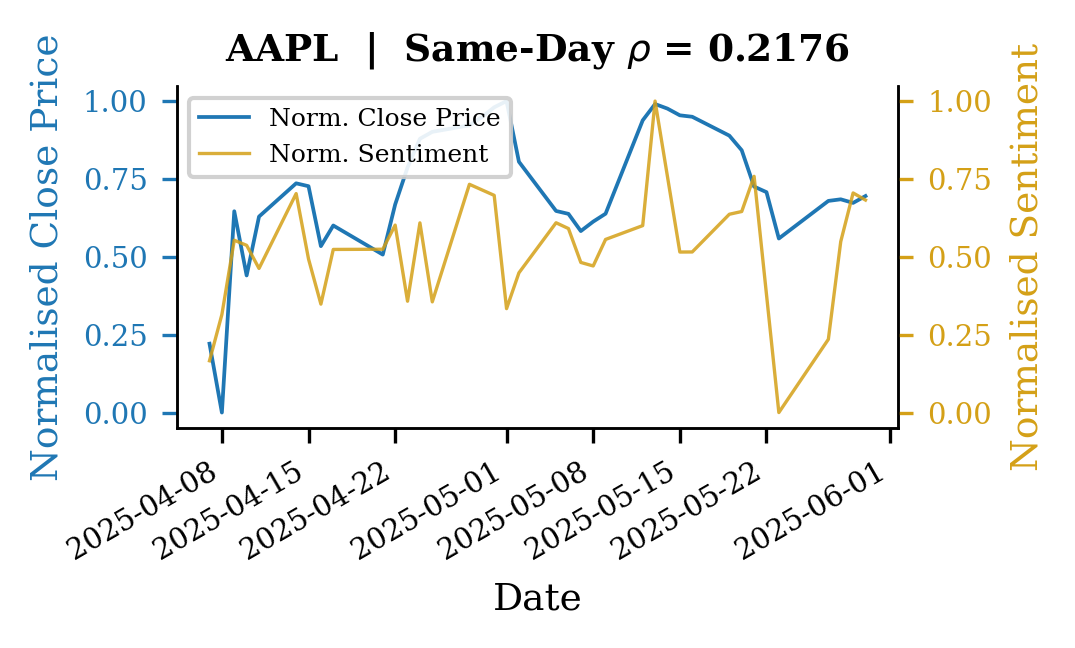
\includegraphics[width=\textwidth]{plots/AAPL_sentiment_price.png}
    \caption{AAPL ($\rho = 0.22$)}
    \label{fig:AAPL_ext}
\end{subfigure}
\hfill
\begin{subfigure}[b]{0.47\textwidth}
    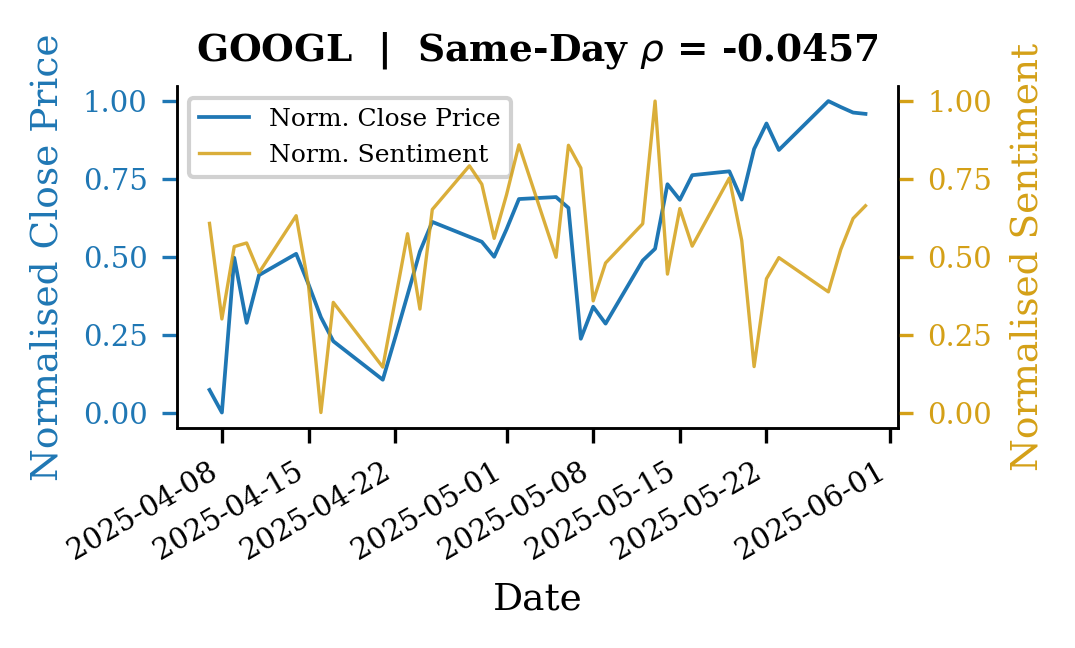
\includegraphics[width=\textwidth]{plots/GOOGL_sentiment_price.png}
    \caption{GOOGL ($\rho = -0.05$)}
    \label{fig:GOOGL_ext}
\end{subfigure}

\vspace{1.0em}

\begin{subfigure}[b]{0.47\textwidth}
    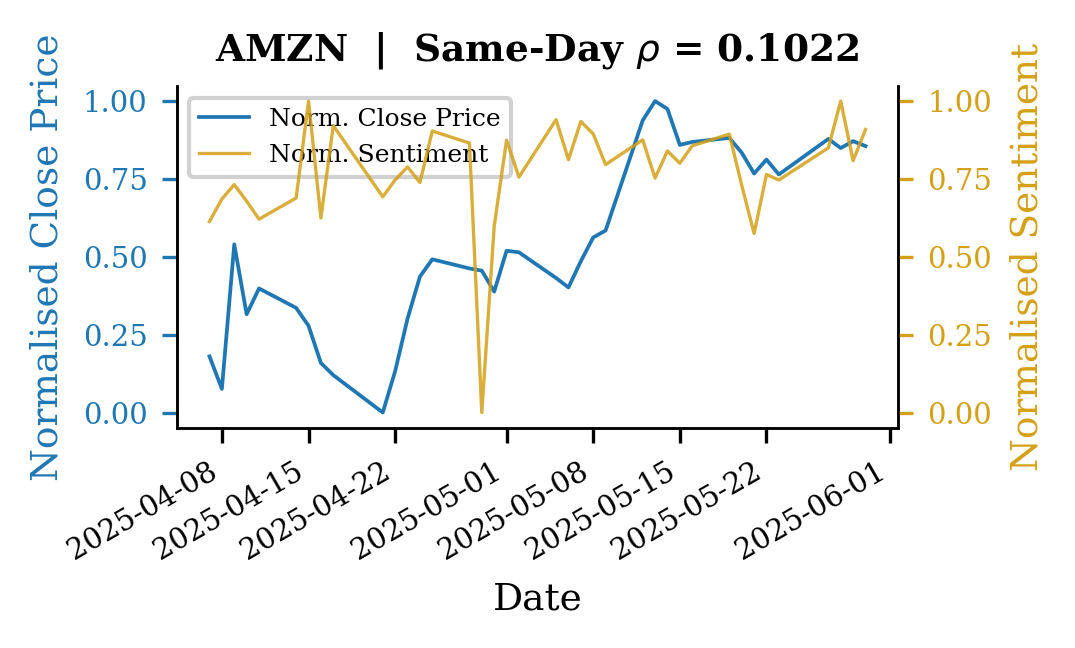
\includegraphics[width=\textwidth]{plots/AMZN_sentiment_price.png}
    \caption{AMZN ($\rho = 0.10$)}
    \label{fig:AMZN_ext}
\end{subfigure}
\hfill
\begin{subfigure}[b]{0.47\textwidth}
    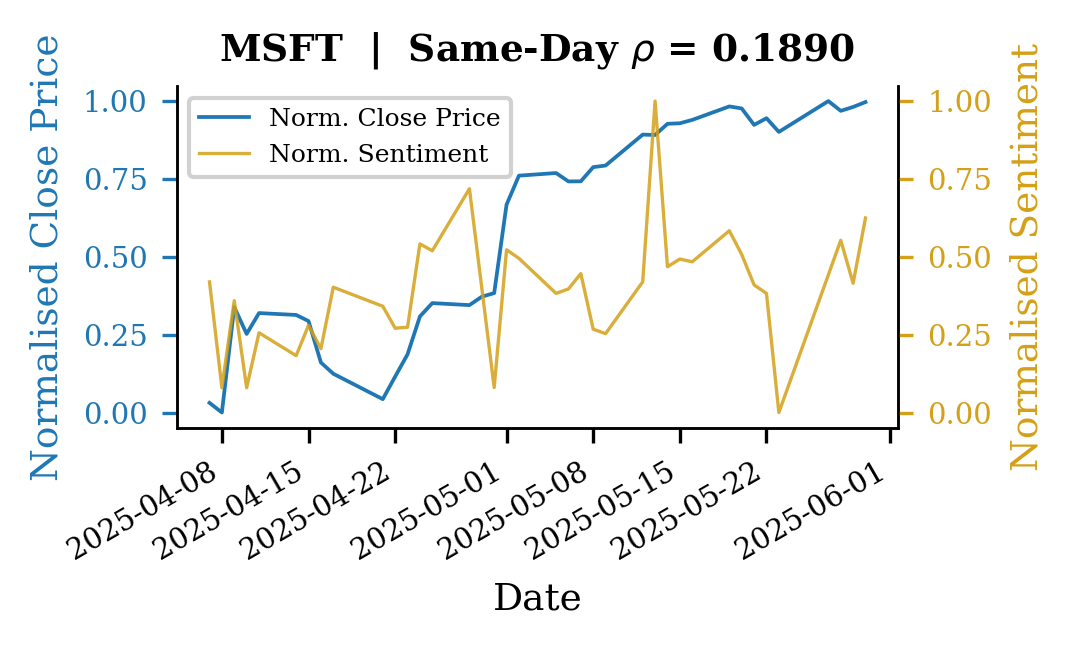
\includegraphics[width=\textwidth]{plots/MSFT_sentiment_price.png}
    \caption{MSFT ($\rho = 0.19$)}
    \label{fig:MSFT_ext}
\end{subfigure}

\vspace{1.0em}

\begin{subfigure}[b]{0.47\textwidth}
    \centering
    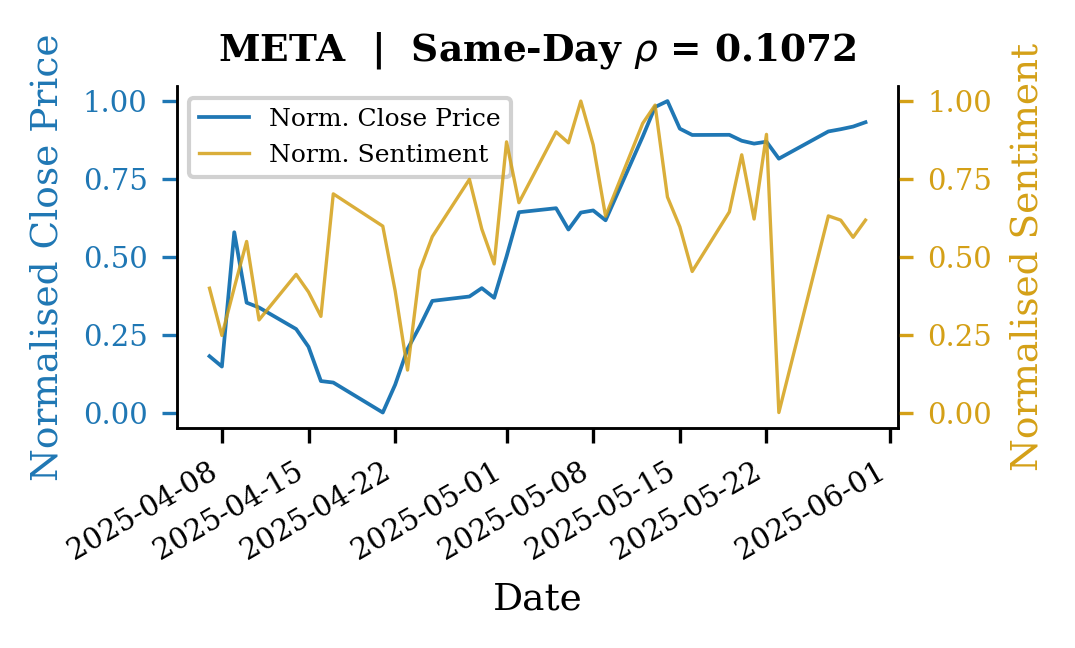
\includegraphics[width=\textwidth]{plots/META_sentiment_price.png}
    \caption{META ($\rho = 0.11$)}
    \label{fig:META_ext}
\end{subfigure}

\caption{Technology sector: normalized closing prices (blue) and normalized daily aggregated sentiment (gold), October 2024--May 2025.}
\label{fig:tech_stocks}
\end{figure*}

\paragraph{Apple (AAPL).}
Apple exhibits moderate positive same-day association ($\rho_{\mathrm{AAPL}} = 0.22$) and a stronger excess-return correlation ($\rho^{\mathrm{ex}} = 0.36$, $p = 0.032$), suggesting that sentiment's relationship with Apple returns is partially masked by broad market movement. The market-controlled regression yields a positive but non-significant lagged sentiment coefficient ($\beta = 0.010$, $p = 0.50$), with the market beta dominating ($\gamma = 1.39$, $p < 0.01$, $R^2 = 0.81$).

\paragraph{Alphabet (GOOGL).}
Alphabet exhibits near-zero same-day association ($\rho_{\mathrm{GOOGL}} = -0.05$) over the extended window, a notable departure from the moderate positive association observed in the original shorter sample. The negative excess-return correlation ($\rho^{\mathrm{ex}} = -0.33$, $p = 0.049$) suggests a possible contrarian pattern during this period. This shift illustrates the sensitivity of sentiment--return relationships to sample window selection.

\paragraph{Amazon (AMZN).}
Amazon exhibits weak positive same-day association ($\rho_{\mathrm{AMZN}} = 0.10$). The regression R\textsuperscript{2} of 0.82 is driven almost entirely by the market factor ($\gamma = 1.27$), with lagged sentiment contributing no additional predictive power ($\beta = 0.013$, $p = 0.35$).

\paragraph{Microsoft (MSFT).}
Microsoft exhibits moderate same-day association ($\rho_{\mathrm{MSFT}} = 0.19$) but a notably significant lag-1 correlation ($\rho^{(1)} = -0.36$, $p = 0.031$), suggesting a reversal pattern: positive sentiment days tend to be followed by negative next-day returns. Most strikingly, Microsoft's extreme-sentiment event analysis yields the strongest result in the sample ($p < 0.001$), with event-day next-day returns averaging 3.7\% compared to a baseline of 0.07\%.

\paragraph{Meta (META).}
Meta exhibits weak positive same-day association ($\rho_{\mathrm{META}} = 0.11$) and a moderate excess-return correlation ($\rho^{\mathrm{ex}} = 0.25$). The market beta ($\gamma = 1.45$) is among the higher values in the technology subsample, consistent with Meta's sensitivity to broad market swings.

\subsubsection{Semiconductors}
Figure~\ref{fig:semi_stocks} shows the semiconductor subsample.

\begin{figure*}[t!]
\centering
\begin{subfigure}[b]{0.47\textwidth}
    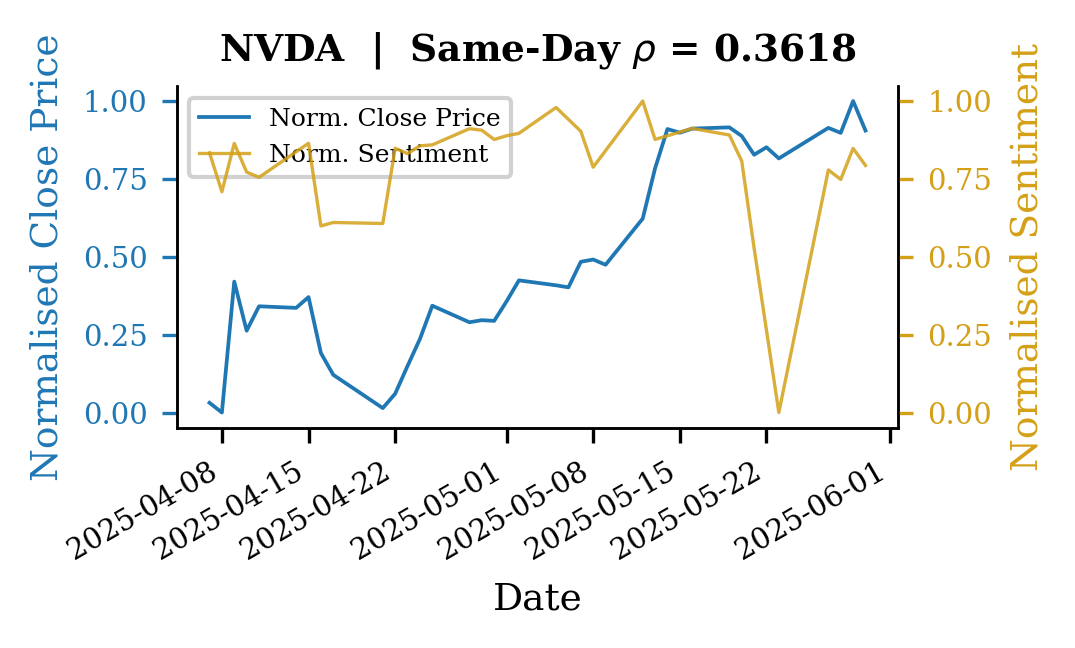
\includegraphics[width=\textwidth]{plots/NVDA_sentiment_price.png}
    \caption{NVDA ($\rho = 0.36$, $p = 0.039$)}
    \label{fig:NVDA_ext}
\end{subfigure}
\hfill
\begin{subfigure}[b]{0.47\textwidth}
    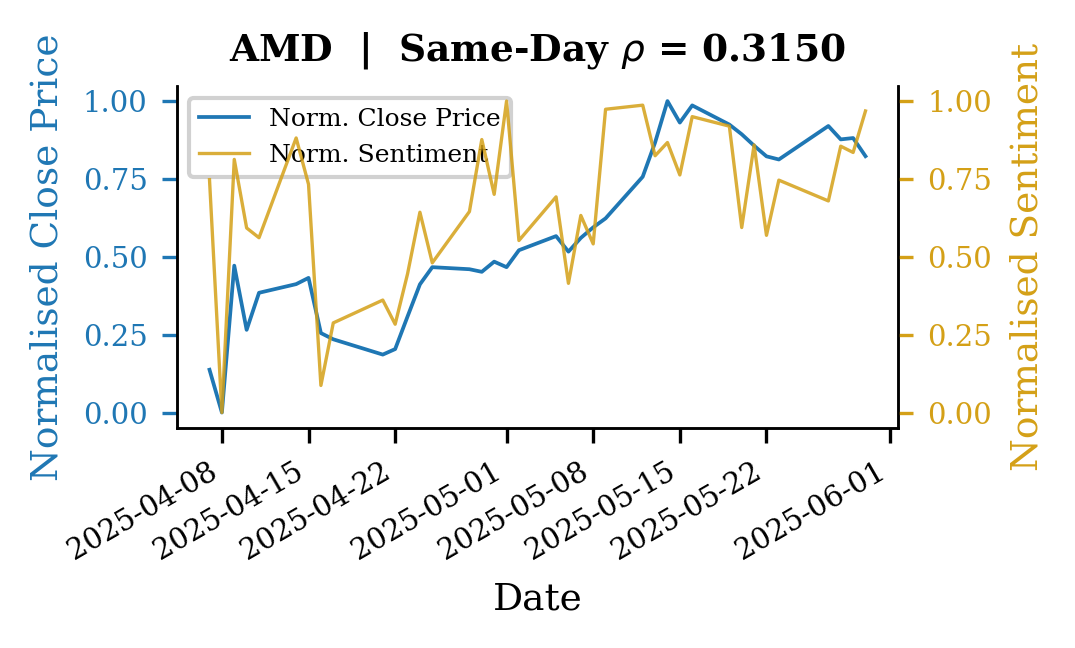
\includegraphics[width=\textwidth]{plots/AMD_sentiment_price.png}
    \caption{AMD ($\rho = 0.31$, $p = 0.054$)}
    \label{fig:AMD_ext}
\end{subfigure}
\caption{Semiconductor sector: normalized closing prices (blue) and normalized daily aggregated sentiment (gold), October 2024--May 2025.}
\label{fig:semi_stocks}
\end{figure*}

\paragraph{Nvidia (NVDA).}
Nvidia exhibits the strongest statistically significant same-day association among all fourteen stocks ($\rho_{\mathrm{NVDA}} = 0.36$, $p = 0.039$), with a similarly strong excess-return correlation ($\rho^{\mathrm{ex}} = 0.34$, $p = 0.052$). The market beta of $\gamma = 1.72$ confirms Nvidia's high sensitivity to broad market movement. These findings are consistent with Nvidia's position as a narrative-driven equity whose valuation is tightly linked to evolving AI expectations.

\paragraph{AMD (AMD).}
AMD exhibits comparable same-day association ($\rho_{\mathrm{AMD}} = 0.31$, $p = 0.054$) and the strongest excess-return correlation in the sample ($\rho^{\mathrm{ex}} = 0.34$, $p = 0.038$). AMD's lag-1 correlation is the most negative in the dataset ($\rho^{(1)} = -0.38$, $p = 0.019$), suggesting a sentiment-reversal pattern. The extreme-sentiment event analysis yields the second most significant result ($p = 0.025$), with event-day next-day returns averaging 5.7\% versus a baseline of 0.16\%. The co-occurrence of strong same-day association and significant event effects in both semiconductor stocks suggests that this sector may be particularly susceptible to sentiment-driven short-horizon dynamics.

\subsubsection{Automotive, Finance, and Other Sectors}
Figure~\ref{fig:other_stocks} shows the remaining seven equities spanning non-technology sectors.

\begin{figure*}[t!]
\centering
\begin{subfigure}[b]{0.32\textwidth}
    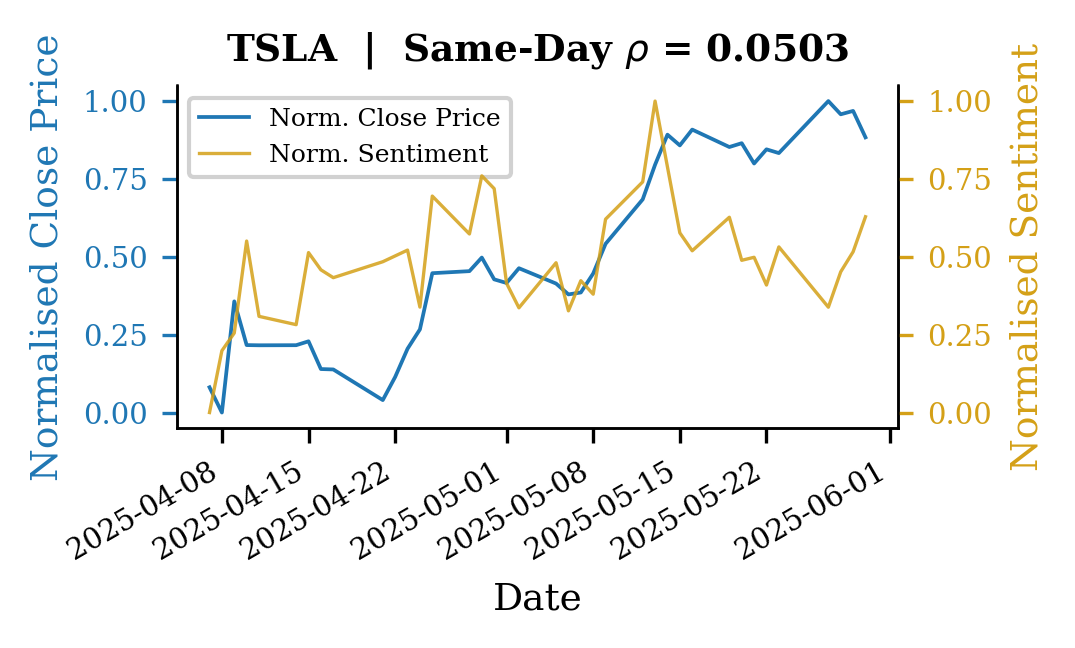
\includegraphics[width=\textwidth]{plots/TSLA_sentiment_price.png}
    \caption{TSLA ($\rho = 0.05$)}
    \label{fig:TSLA_ext}
\end{subfigure}
\hfill
\begin{subfigure}[b]{0.32\textwidth}
    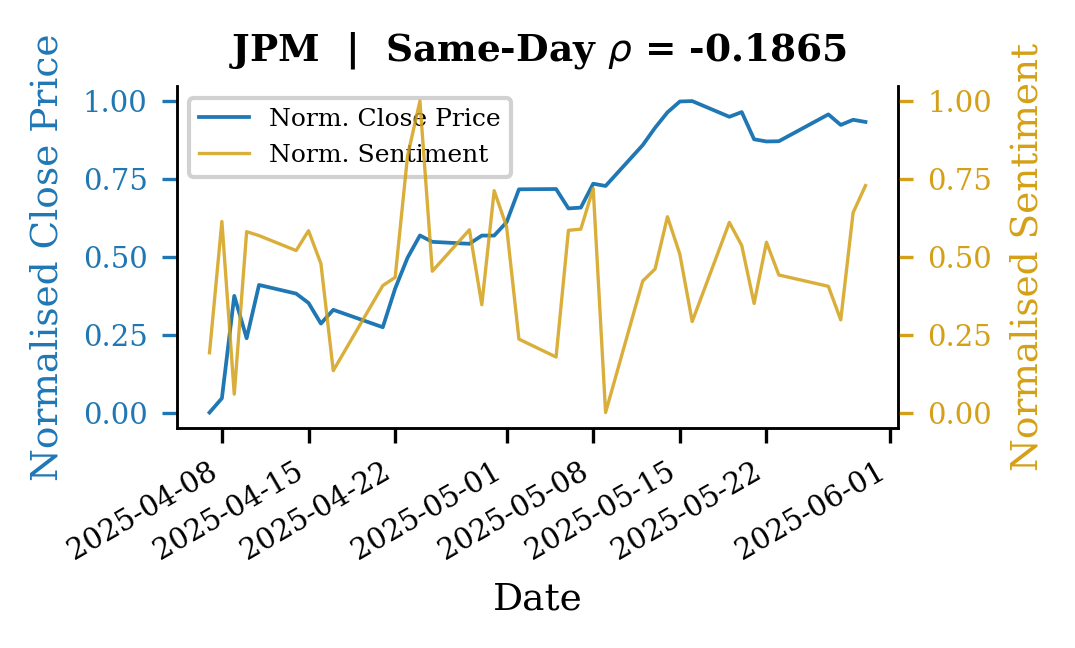
\includegraphics[width=\textwidth]{plots/JPM_sentiment_price.png}
    \caption{JPM ($\rho = -0.19$)}
    \label{fig:JPM_ext}
\end{subfigure}
\hfill
\begin{subfigure}[b]{0.32\textwidth}
    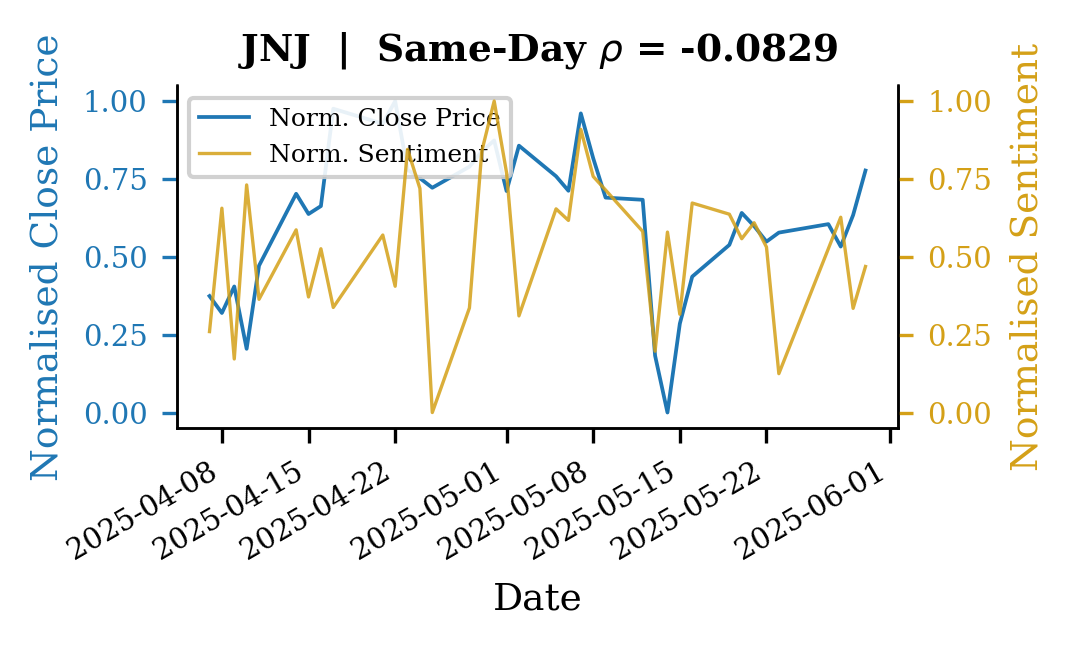
\includegraphics[width=\textwidth]{plots/JNJ_sentiment_price.png}
    \caption{JNJ ($\rho = -0.08$)}
    \label{fig:JNJ_ext}
\end{subfigure}

\vspace{1.0em}

\begin{subfigure}[b]{0.32\textwidth}
    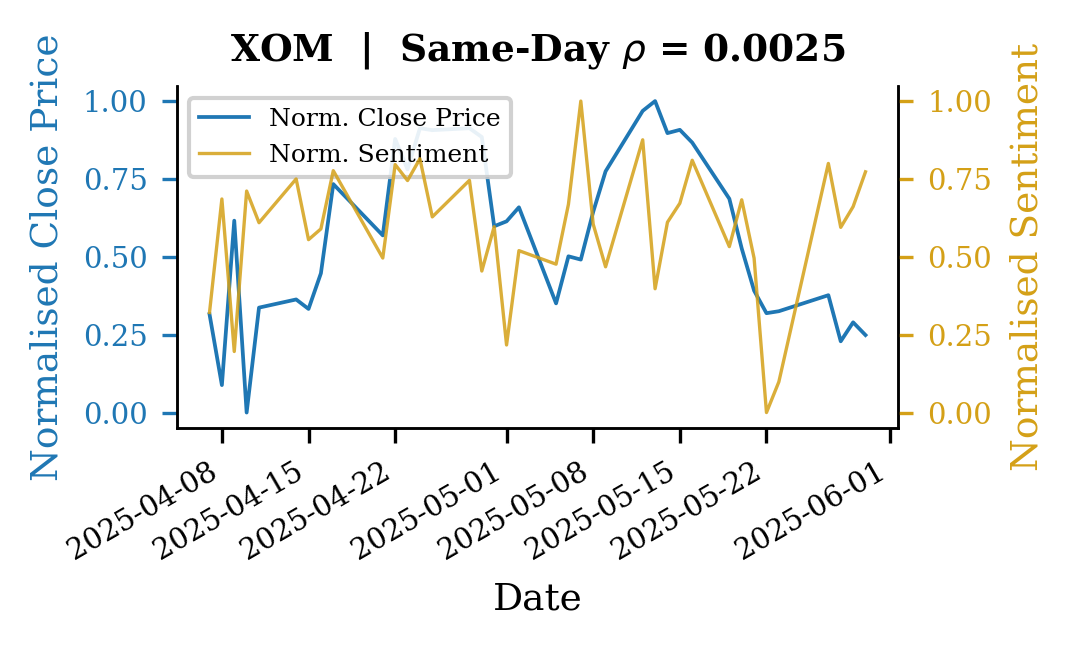
\includegraphics[width=\textwidth]{plots/XOM_sentiment_price.png}
    \caption{XOM ($\rho = 0.00$)}
    \label{fig:XOM_ext}
\end{subfigure}
\hfill
\begin{subfigure}[b]{0.32\textwidth}
    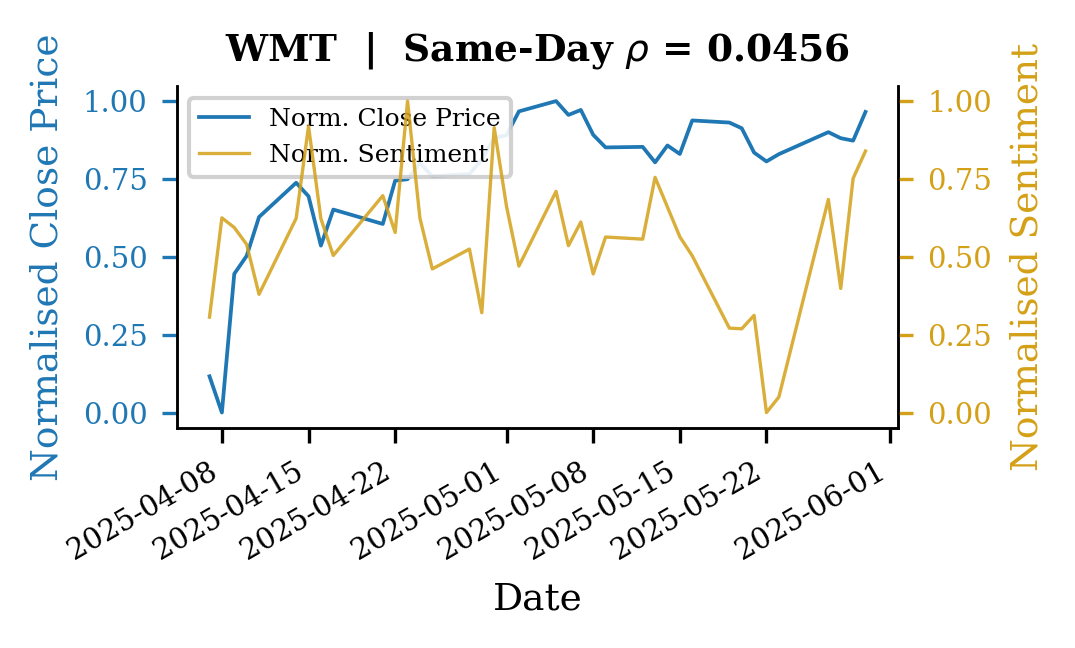
\includegraphics[width=\textwidth]{plots/WMT_sentiment_price.png}
    \caption{WMT ($\rho = 0.05$)}
    \label{fig:WMT_ext}
\end{subfigure}
\hfill
\begin{subfigure}[b]{0.32\textwidth}
    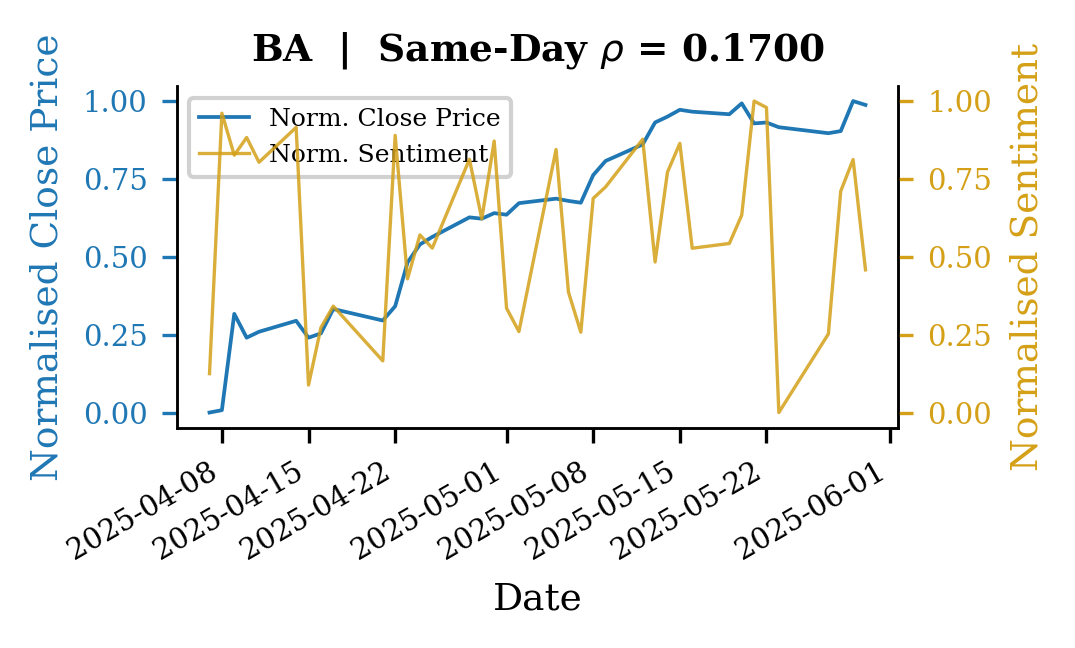
\includegraphics[width=\textwidth]{plots/BA_sentiment_price.png}
    \caption{BA ($\rho = 0.17$)}
    \label{fig:BA_ext}
\end{subfigure}

\vspace{1.0em}

\begin{subfigure}[b]{0.32\textwidth}
    \centering
    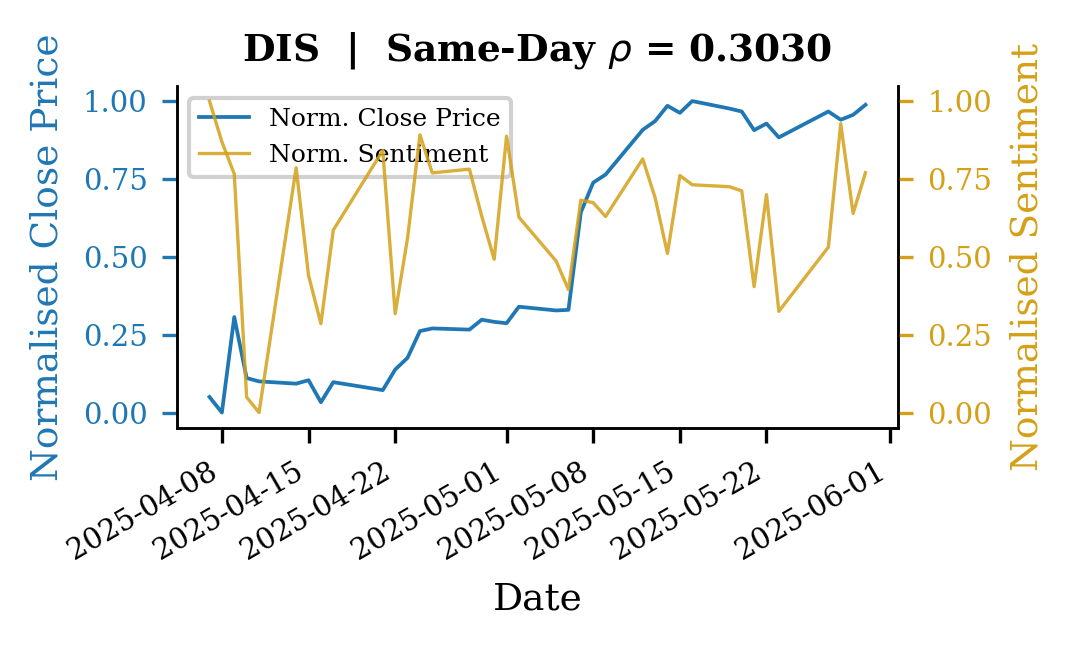
\includegraphics[width=\textwidth]{plots/DIS_sentiment_price.png}
    \caption{DIS ($\rho = 0.30$)}
    \label{fig:DIS_ext}
\end{subfigure}

\caption{Non-technology sectors: normalized closing prices (blue) and normalized daily aggregated sentiment (gold), October 2024--May 2025.}
\label{fig:other_stocks}
\end{figure*}

\paragraph{Tesla (TSLA).}
Tesla continues to exhibit near-zero same-day association ($\rho_{\mathrm{TSLA}} = 0.05$) despite having the second-highest article volume in the expanded sample. The market beta of $\gamma = 2.04$---the highest in the dataset---indicates extreme sensitivity to broad market movements, which may dominate any sentiment signal. The combination of very high media volume, high market beta, and near-zero sentiment association is consistent with the saturation and noise-discounting interpretation discussed in Section~\ref{sec:preliminaries}.

\paragraph{JPMorgan (JPM).}
JPMorgan exhibits negative same-day association ($\rho_{\mathrm{JPM}} = -0.19$), the most negative raw correlation in the sample. This is consistent with a financial-sector information environment in which institutional investors process news through quantitative models rather than emotional heuristics, potentially producing contrarian trading patterns relative to media tone. The significant lag-2 correlation ($\rho^{(2)} = -0.36$, $p = 0.033$) suggests a delayed reversal effect.

\paragraph{Johnson \& Johnson (JNJ).}
Johnson \& Johnson exhibits near-zero same-day association ($\rho_{\mathrm{JNJ}} = -0.08$) and, uniquely in the sample, a non-significant market beta ($\gamma = 0.12$, $p = 0.23$, $R^2 = 0.04$). This extreme decoupling from both market movement and media sentiment is consistent with JNJ's status as a defensive healthcare stock whose valuation is driven primarily by dividend yield, patent pipeline, and regulatory outcomes rather than short-horizon narrative dynamics.

\paragraph{ExxonMobil (XOM).}
ExxonMobil exhibits near-zero same-day association ($\rho_{\mathrm{XOM}} = 0.00$). Energy-sector returns are driven primarily by commodity price movements, OPEC decisions, and geopolitical events, which may decouple stock behavior from the general emotional tone of company-specific media coverage.

\paragraph{Walmart (WMT).}
Walmart exhibits near-zero same-day association ($\rho_{\mathrm{WMT}} = 0.05$). Consumer staples stocks are typically held for yield and stability; the investor base may be less responsive to sentiment-driven narratives.

\paragraph{Boeing (BA).}
Boeing exhibits weak positive same-day association ($\rho_{\mathrm{BA}} = 0.17$) but a notably strong negative lag-2 correlation ($\rho^{(2)} = -0.46$, $p = 0.005$), the largest lagged effect in the sample. This delayed reversal may reflect Boeing's event-driven news environment, where initial sentiment shocks (e.g., safety incidents, contract announcements) are followed by mean-reverting return dynamics as more complete information becomes available.

\paragraph{Disney (DIS).}
Disney exhibits moderate positive same-day association ($\rho_{\mathrm{DIS}} = 0.30$, $p = 0.065$), the highest among non-technology, non-semiconductor stocks. As a media and entertainment company, Disney's valuation may be more narrative-sensitive than other non-technology firms, bridging the gap between technology-sector dynamics and traditional industrials.

\subsubsection{Cross-Sector Comparison}
Figure~\ref{fig:volumesent} depicts media volume versus descriptive sentiment--return association for all fourteen equities, color-coded by sector. Figure~\ref{fig:sector_heatmap} provides a heatmap of all association measures across the full sample. Figure~\ref{fig:market_betas} compares the market sensitivity ($\gamma_k$) coefficients across equities, revealing a spectrum from JNJ's near-zero market coupling to Tesla's extreme market beta.

\begin{figure*}[t!]
    \centering
    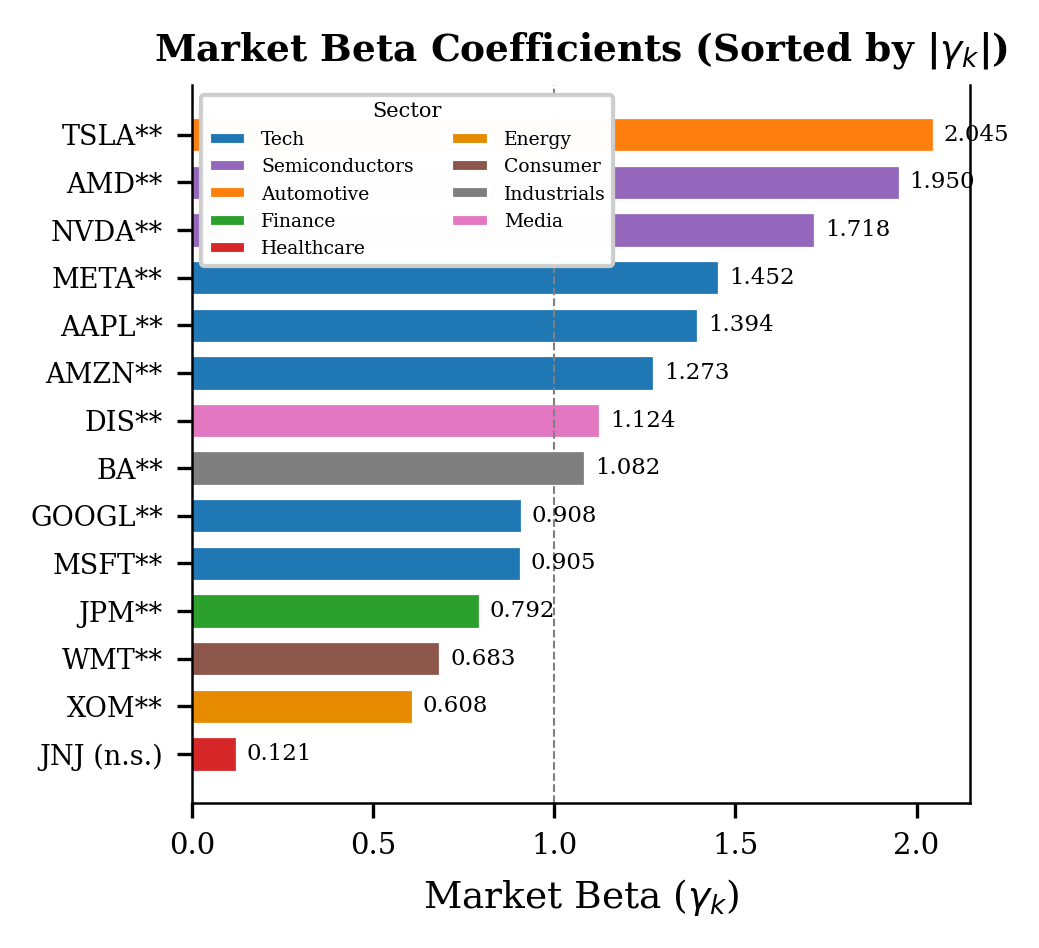
\includegraphics[width=.85\linewidth]{plots/market_betas.png}
    \caption{Market sensitivity coefficients ($\gamma_k$) from the lagged market-controlled regression for all fourteen equities. Higher values indicate greater sensitivity to broad market movement. All coefficients are significant at $p < 0.01$ except JNJ ($p = 0.23$).}
    \label{fig:market_betas}
\end{figure*}

\begin{figure*}[t!]
    \centering
    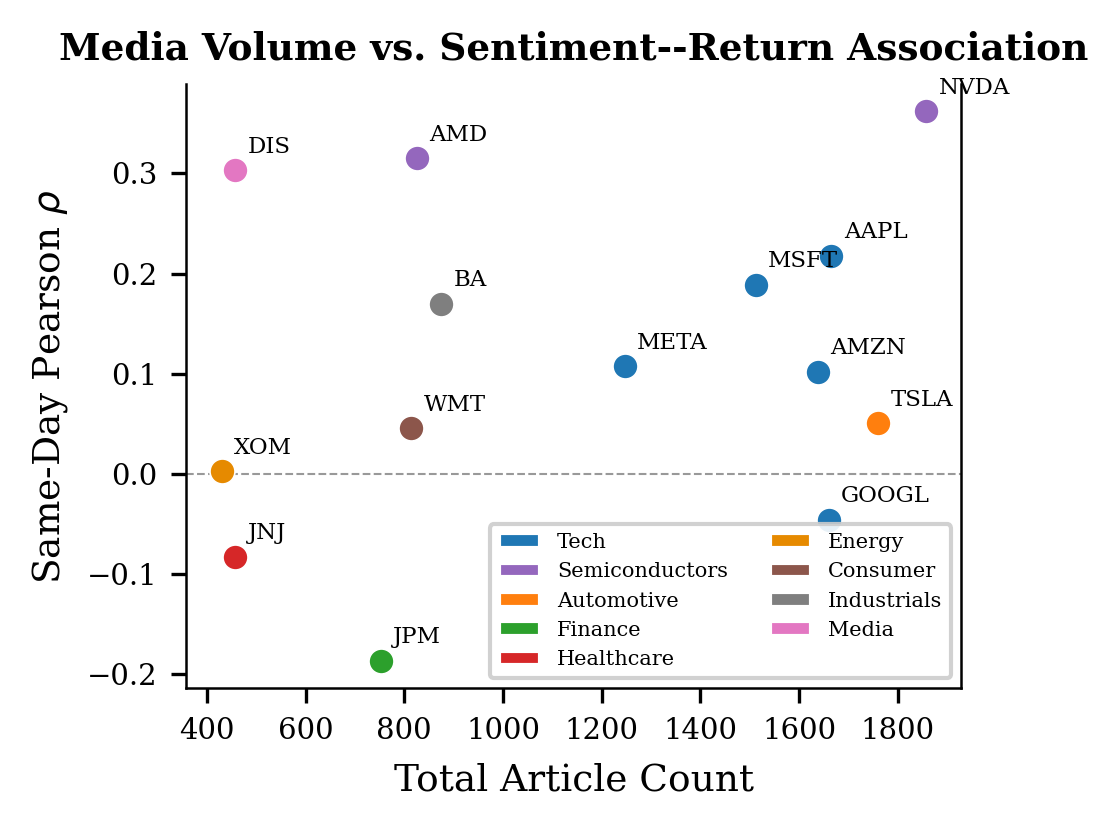
\includegraphics[width=.8\linewidth]{plots/volume_vs_association.png}
    \caption{Media volume vs.\ descriptive sentiment--return association for fourteen equities, color-coded by sector. Semiconductor stocks (NVDA, AMD) cluster in the upper portion despite moderate volume, while Tesla exhibits high volume with near-zero association.}
    \label{fig:volumesent}
\end{figure*}

\begin{figure*}[t!]
    \centering
    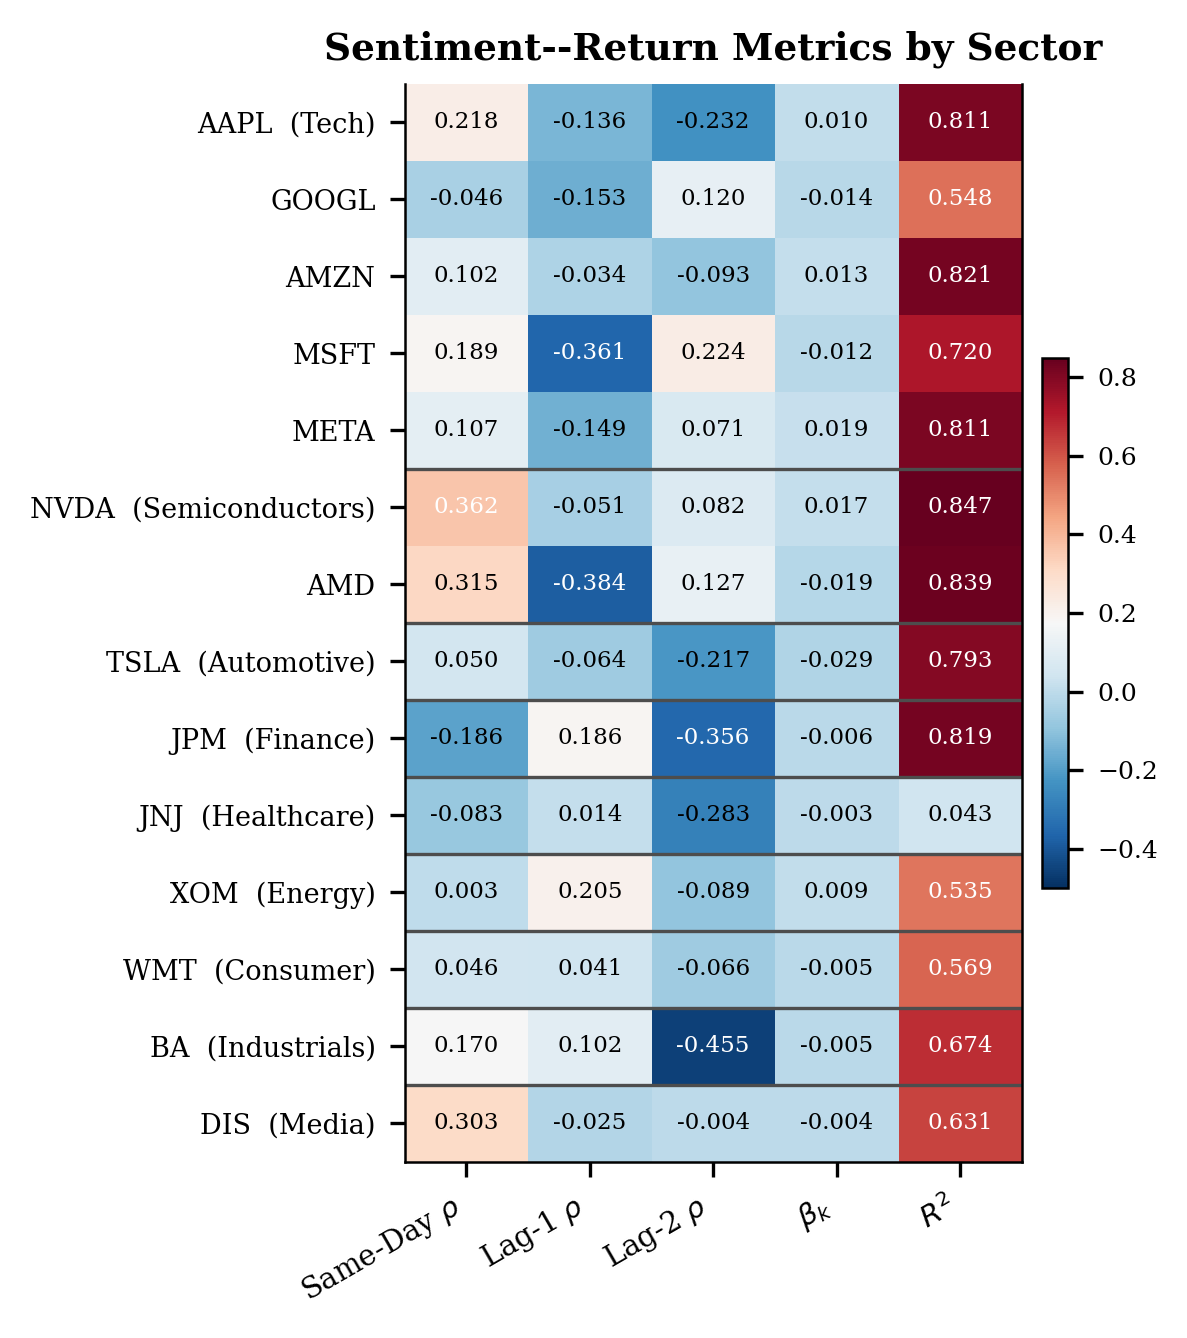
\includegraphics[width=.95\linewidth]{plots/sector_heatmap.png}
    \caption{Heatmap of sentiment--return association measures across fourteen equities grouped by sector. Warmer colors indicate stronger positive association; cooler colors indicate negative association.}
    \label{fig:sector_heatmap}
\end{figure*}

\subsection{Sentiment--Price Alignment Classification}

To provide a practical summary of how closely each stock's price movements track media sentiment, we classify the fourteen equities into three alignment tiers based on the magnitude of the same-day Pearson correlation and the excess-return correlation. Table~\ref{tab:alignment} reports these classifications alongside both raw and market-adjusted correlations.

\begin{table*}[t!]
\centering
\caption{Sentiment--Price Alignment Classification. $\rho$ denotes same-day Pearson correlation between daily aggregated sentiment and daily log returns. $\rho^{\mathrm{ex}}$ denotes the correlation with excess returns (stock return minus SPY return). Alignment tiers: \textbf{Strong} ($|\rho| \geq 0.30$), \textbf{Moderate} ($0.15 \leq |\rho| < 0.30$), \textbf{Weak} ($|\rho| < 0.15$).}
\label{tab:alignment}
\begin{tabular}{llccccl}
\toprule
\textbf{Sector} & \textbf{Stock} & \textbf{$\rho$} & \textbf{$p$-value} & \textbf{$\rho^{\mathrm{ex}}$} & \textbf{$p$-value} & \textbf{Alignment} \\
\midrule
\multirow{5}{*}{Tech}  & AAPL  & $+0.22$ & $0.209$ & $+0.36$ & $0.032^{*}$ & Moderate \\
                        & GOOGL & $-0.05$ & $0.788$ & $-0.33$ & $0.049^{*}$ & Weak \\
                        & AMZN  & $+0.10$ & $0.541$ & $+0.13$ & $0.422$ & Weak \\
                        & MSFT  & $+0.19$ & $0.263$ & $+0.06$ & $0.723$ & Moderate \\
                        & META  & $+0.11$ & $0.522$ & $+0.25$ & $0.123$ & Weak \\
\midrule
\multirow{2}{*}{Semi}  & NVDA  & $+0.36$ & $0.039^{*}$ & $+0.34$ & $0.052^{\dagger}$ & Strong \\
                        & AMD   & $+0.32$ & $0.054^{\dagger}$ & $+0.34$ & $0.038^{*}$ & Strong \\
\midrule
Auto   & TSLA  & $+0.05$ & $0.771$ & $+0.16$ & $0.347$ & Weak \\
\midrule
Finance & JPM  & $-0.19$ & $0.262$ & $+0.06$ & $0.734$ & Moderate \\
\midrule
Health & JNJ   & $-0.08$ & $0.621$ & $+0.20$ & $0.228$ & Weak \\
\midrule
Energy & XOM   & $+0.00$ & $0.988$ & $+0.11$ & $0.515$ & Weak \\
\midrule
Consumer & WMT & $+0.05$ & $0.789$ & $-0.07$ & $0.677$ & Weak \\
\midrule
Industrial & BA & $+0.17$ & $0.307$ & $+0.13$ & $0.439$ & Moderate \\
\midrule
Media  & DIS   & $+0.30$ & $0.065^{\dagger}$ & $+0.23$ & $0.168$ & Strong \\
\bottomrule
\multicolumn{7}{l}{\small $^{*}p < 0.05$; $^{\dagger}p < 0.10$}
\end{tabular}
\end{table*}

Three patterns emerge from the alignment classification:

\begin{itemize}
    \item \textbf{Strong alignment} (NVDA, AMD, DIS): These equities exhibit same-day correlations of $|\rho| \geq 0.30$, and the semiconductor stocks maintain this alignment even after removing market-wide movement. These are \textit{narrative-sensitive} stocks whose valuations depend heavily on forward-looking stories (AI growth for semiconductors, streaming dynamics for Disney) and that attract substantial retail investor participation.

    \item \textbf{Moderate alignment} (AAPL, MSFT, JPM, BA): These equities show correlations in the $0.15$--$0.30$ range. Notably, Apple's alignment strengthens substantially when measured against excess returns ($\rho^{\mathrm{ex}} = +0.36$, $p = 0.032$), suggesting that its sentiment--return link is partially masked by broad market movement. JPMorgan's negative raw correlation ($\rho = -0.19$) vanishes after market adjustment ($\rho^{\mathrm{ex}} = +0.06$), indicating that its apparent contrarian pattern is an artifact of market-wide dynamics rather than a genuine sentiment effect.

    \item \textbf{Weak alignment} (GOOGL, AMZN, META, TSLA, JNJ, XOM, WMT): These equities show $|\rho| < 0.15$, indicating that media sentiment has little observable relationship with their short-horizon price movements. For TSLA, this is consistent with the noise-discounting interpretation: despite the second-highest media volume, the stock's price behavior is dominated by its extreme market beta ($\gamma = 2.04$) rather than sentiment signals. For JNJ, XOM, and WMT, the weak alignment reflects sector-specific information environments in which returns are driven by factors orthogonal to media tone.
\end{itemize}

The alignment classification provides a practical framework for assessing which equities may be more susceptible to sentiment-driven price dynamics and, by extension, to potential manipulation through coordinated media narratives. Strong-alignment stocks represent the highest-priority targets for the sentiment anomaly monitoring system described in Section~\ref{sec:data_method}.

\subsection{Lagged Association Results}
Table~\ref{tab:lagged_results} reports same-day and lagged sentiment--return associations for each stock. Compared with contemporaneous correlation, the lagged estimates provide a clearer view of whether sentiment precedes subsequent return behavior.

\begin{table}[!htbp]
\centering
\caption{Same-Day and Lagged Sentiment--Return Associations}
\label{tab:lagged_results}
\begin{tabular}{llccc}
\toprule
\textbf{Sector} & \textbf{Stock} & \textbf{Same-Day $\rho$} & \textbf{Lag-1 $\rho^{(1)}$} & \textbf{Lag-2 $\rho^{(2)}$} \\
\midrule
\multirow{5}{*}{Tech}  & AAPL  & $0.22$ & $-0.14$ & $-0.23$ \\
                        & GOOGL & $-0.05$ & $-0.15$ & $0.12$ \\
                        & AMZN  & $0.10$ & $-0.03$ & $-0.09$ \\
                        & MSFT  & $0.19$ & $-0.36^{*}$ & $0.22$ \\
                        & META  & $0.11$ & $-0.15$ & $0.07$ \\
\midrule
\multirow{2}{*}{Semi}  & NVDA  & $0.36^{*}$ & $-0.05$ & $0.08$ \\
                        & AMD   & $0.31^{\dagger}$ & $-0.38^{*}$ & $0.13$ \\
\midrule
Auto   & TSLA  & $0.05$ & $-0.06$ & $-0.22$ \\
\midrule
Finance & JPM  & $-0.19$ & $0.19$ & $-0.36^{*}$ \\
\midrule
Health & JNJ   & $-0.08$ & $0.01$ & $-0.28^{\dagger}$ \\
\midrule
Energy & XOM   & $0.00$ & $0.20$ & $-0.09$ \\
\midrule
Consumer & WMT & $0.05$ & $0.04$ & $-0.07$ \\
\midrule
Industrial & BA & $0.17$ & $0.10$ & $-0.46^{*}$ \\
\midrule
Media  & DIS   & $0.30^{\dagger}$ & $-0.03$ & $-0.00$ \\
\bottomrule
\multicolumn{5}{l}{\small $^{*}p < 0.05$; $^{\dagger}p < 0.10$}
\end{tabular}
\end{table}


\subsection{Market-Controlled Regression Results}
Table~\ref{tab:regression_results} reports the lagged market-controlled regressions. The coefficient on lagged sentiment, $\beta_k$, indicates whether next-day returns remain associated with prior-day sentiment after controlling for broad market movement.

\begin{table}[!htbp]
\centering
\caption{Lagged Market-Controlled Regression Results}
\label{tab:regression_results}
\begin{tabular}{llccc}
\toprule
\textbf{Sector} & \textbf{Stock} & \textbf{$\beta_k$ on $S_{k,t-1}$} & \textbf{$\gamma_k$ on $r_{m,t}$} & \textbf{$R^2$} \\
\midrule
\multirow{5}{*}{Tech}  & AAPL  & $0.010$ & $1.394^{*}$ & $0.811$ \\
                        & GOOGL & $-0.014$ & $0.908^{*}$ & $0.548$ \\
                        & AMZN  & $0.013$ & $1.273^{*}$ & $0.821$ \\
                        & MSFT  & $-0.012$ & $0.905^{*}$ & $0.720$ \\
                        & META  & $0.019$ & $1.452^{*}$ & $0.811$ \\
\midrule
\multirow{2}{*}{Semi}  & NVDA  & $0.017$ & $1.718^{*}$ & $0.847$ \\
                        & AMD   & $-0.019$ & $1.950^{*}$ & $0.839$ \\
\midrule
Auto   & TSLA  & $-0.029$ & $2.045^{*}$ & $0.793$ \\
\midrule
Finance & JPM  & $-0.006$ & $0.792^{*}$ & $0.819$ \\
\midrule
Health & JNJ   & $-0.003$ & $0.121$ & $0.043$ \\
\midrule
Energy & XOM   & $0.009$ & $0.608^{*}$ & $0.536$ \\
\midrule
Consumer & WMT & $-0.005$ & $0.683^{*}$ & $0.569$ \\
\midrule
Industrial & BA & $-0.005$ & $1.082^{*}$ & $0.675$ \\
\midrule
Media  & DIS   & $-0.004$ & $1.124^{*}$ & $0.631$ \\
\bottomrule
\multicolumn{5}{l}{\small $^{*}p < 0.01$}
\end{tabular}
\end{table}


\subsection{Extreme-Sentiment Event Results}
We next examine whether extreme sentiment realizations are followed by distinguishable next-day return behavior. Table~\ref{tab:event_results} compares the mean next-day return following extreme-sentiment days with the baseline mean next-day return for non-event days.

\begin{table*}[t!]
\centering
\caption{Extreme-Sentiment Event Analysis. Boldface indicates statistically significant event--baseline differences.}
\label{tab:event_results}
\begin{tabular}{llcccc}
\toprule
\textbf{Sector} & \textbf{Stock} & \textbf{Threshold} & \textbf{$n_{\mathrm{events}}$} & \textbf{Mean Next-Day (Event)} & \textbf{Mean Next-Day (Baseline)} \\
\midrule
\multirow{5}{*}{Tech}  & AAPL  & $|\tilde{S}| > 1.5$ & 4 & $-0.0073$ & $0.0044$ \\
                        & GOOGL & $|\tilde{S}| > 1.5$ & 6 & $-0.0023$ & $0.0049$ \\
                        & AMZN  & $|\tilde{S}| > 1.0$ & 5 & $-0.0001$ & $0.0049$ \\
                        & \textbf{MSFT}  & $|\tilde{S}| > 1.5$ & 6 & $\mathbf{0.0372}$ & $\mathbf{0.0007}$ \\
                        & META  & $|\tilde{S}| > 1.5$ & 4 & $0.0139$ & $0.0052$ \\
\midrule
\multirow{2}{*}{Semi}  & NVDA  & $|\tilde{S}| > 1.0$ & 7 & $0.0072$ & $0.0094$ \\
                        & \textbf{AMD}   & $|\tilde{S}| > 1.5$ & 4 & $\mathbf{0.0573}$ & $\mathbf{0.0016}$ \\
\midrule
Auto   & TSLA  & $|\tilde{S}| > 1.5$ & 4 & $0.0264$ & $0.0066$ \\
\midrule
Finance & JPM  & $|\tilde{S}| > 1.5$ & 5 & $-0.0012$ & $0.0067$ \\
\midrule
Health & JNJ   & $|\tilde{S}| > 1.5$ & 5 & $-0.0061$ & $0.0019$ \\
\midrule
Energy & XOM   & $|\tilde{S}| > 1.5$ & 5 & $-0.0068$ & $0.0009$ \\
\midrule
Consumer & WMT & $|\tilde{S}| > 1.5$ & 5 & $-0.0004$ & $0.0050$ \\
\midrule
Industrial & BA & $|\tilde{S}| > 1.5$ & 4 & $0.0058$ & $0.0114$ \\
\midrule
Media  & DIS   & $|\tilde{S}| > 1.5$ & 3 & $-0.0086$ & $0.0097$ \\
\bottomrule
\end{tabular}
\end{table*}

\begin{figure*}[t!]
    \centering
    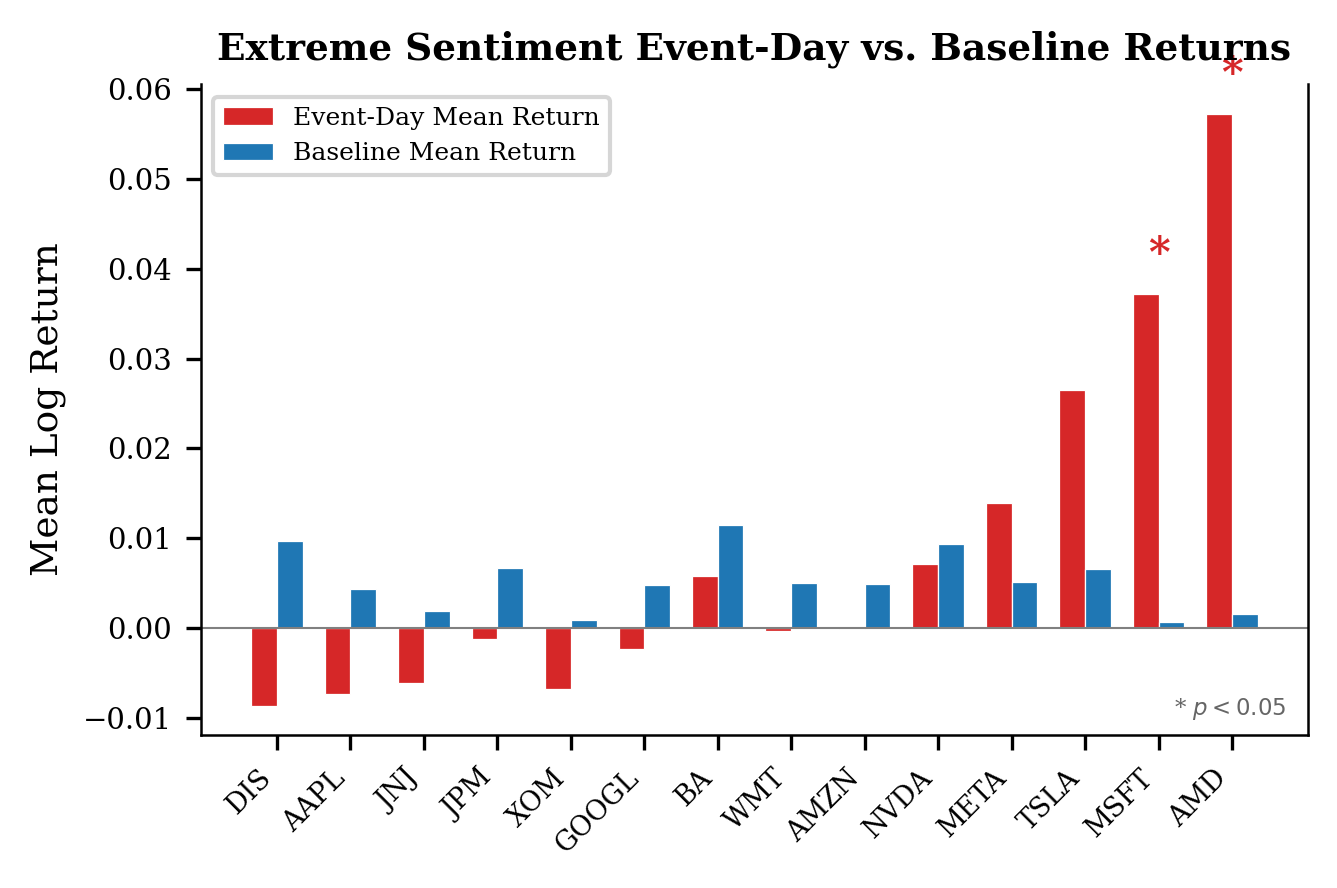
\includegraphics[width=.85\linewidth]{plots/extreme_events.png}
    \caption{Extreme-sentiment event analysis: mean next-day return for event days (dark bars) vs.\ baseline non-event days (light bars). Stars indicate statistically significant differences (MSFT: $p < 0.001$; AMD: $p = 0.025$).}
    \label{fig:extreme_events}
\end{figure*}


\subsection{Summary Typology}
Table~\ref{tab:typology_main2} summarizes the restrained descriptive typology used in this paper.

\begin{table}[!htbp]
\centering
\caption{Descriptive Typology of Observed Sentiment Association}
\label{tab:typology_main2}
\begin{tabular}{|p{0.19\linewidth}|p{0.21\linewidth}|p{0.40\linewidth}|}
\hline
\textbf{Range} & \textbf{Label} & \textbf{Interpretation} \\
\hline
$[0.30, 0.70)$ & Moderate Sentiment Association (MSA) & Daily aggregated sentiment and daily log returns exhibit moderate positive descriptive co-movement during the study window. \\
\hline
$(-0.30, 0.30)$ & Low Sentiment Association (LSA) & Daily aggregated sentiment and daily log returns exhibit weak descriptive co-movement during the study window. \\
\hline
\end{tabular}
\end{table}

In the expanded sample, Nvidia ($\rho = 0.36$), AMD ($\rho = 0.31$), and Disney ($\rho = 0.30$) fall into or near the MSA range. The remaining eleven equities fall into the LSA range, with JPMorgan ($\rho = -0.19$) and JNJ ($\rho = -0.08$) exhibiting negative same-day association. This distribution suggests that meaningful same-day sentiment--return co-movement is concentrated in narrative-driven sectors (semiconductors, media/entertainment) rather than being a universal feature of highly visible equities.

\section{Discussion}
\label{sec:discussion}

\subsection{Interpreting Heterogeneity Across Fourteen Stocks}
The fourteen case studies confirm and extend the central finding from the original five-stock pilot: media sentiment is not equally related to short-horizon returns across equities, and this heterogeneity varies systematically across sectors. The expanded sample reveals three distinct behavioral regimes.

\paragraph{Regime 1: Narrative-sensitive equities.}
Semiconductor stocks (NVDA, AMD) and Disney exhibit the strongest same-day sentiment--return association ($\rho \geq 0.30$). These equities share two features: (a) their valuations are tightly linked to forward-looking narratives (AI growth expectations for semiconductors, streaming subscriber dynamics for Disney), and (b) they attract substantial retail investor participation, a population more likely to engage in System 1 processing of emotionally salient headlines \cite{kahneman2011thinking, barber2008all}. The co-occurrence of strong same-day association and significant extreme-sentiment event effects in both semiconductor stocks provides converging evidence for sentiment-linked return dynamics in this sector.

\paragraph{Regime 2: Market-dominated equities.}
Most technology stocks (AAPL, AMZN, MSFT, META) and Boeing exhibit moderate but non-significant same-day association ($0.10 \leq |\rho| \leq 0.22$). For these equities, the market factor ($\gamma_k$) dominates the regression, with $R^2$ values exceeding 0.67 driven almost entirely by broad market movement. Lagged sentiment adds minimal explanatory power ($\beta_k$ non-significant in all cases). This pattern suggests that these stocks are sufficiently diversified in their investor base and information environment that media sentiment signals are subsumed by market-wide dynamics.

\paragraph{Regime 3: Sentiment-decoupled equities.}
Non-technology sectors---JPMorgan, JNJ, ExxonMobil, Walmart---exhibit near-zero or negative same-day association. JNJ's near-zero $R^2$ in the market-controlled regression ($R^2 = 0.04$) is particularly striking: it is essentially uncorrelated with both market movement and media sentiment. This decoupling is consistent with a sector-specific information environment in which returns are driven by factors orthogonal to media tone---commodity prices (XOM), regulatory outcomes (JNJ), macroeconomic conditions (JPM), and consumer spending patterns (WMT).

A cautious behavioral interpretation is that differences in observed association may reflect some combination of the following:
\begin{itemize}
    \item \textbf{Sector-specific information environments}: the degree to which firm value is tied to narratives versus fundamentals;
    \item \textbf{Investor composition}: the proportion of retail versus institutional investors, and the degree of commitment or contrarianism in the investor base;
    \item \textbf{Media saturation}: the extent to which high media volume reduces the marginal informativeness of additional coverage;
    \item \textbf{Narrative polarization}: the degree to which competing positive and negative narratives cancel out in daily aggregation;
    \item \textbf{Market beta}: the extent to which broad market movement dominates firm-specific dynamics.
\end{itemize}

\paragraph{Tesla revisited.}
Tesla continues to exhibit near-zero sentiment association ($\rho = 0.05$) despite having the second-highest article volume (1{,}760 articles) and the highest market beta ($\gamma = 2.04$). The expanded cross-sector analysis strengthens the interpretation that Tesla's anomalous pattern reflects a combination of media saturation, narrative polarization, and a committed investor base that discounts emotionally framed coverage as noise. Notably, Tesla's extreme-sentiment event analysis shows a positive but non-significant event effect (event mean $= 0.026$, baseline $= 0.007$, $p = 0.47$), suggesting that even large sentiment shocks do not reliably predict next-day return behavior for this equity.

\paragraph{The Microsoft--AMD anomaly.}
The most striking finding in the expanded sample is the statistically significant extreme-sentiment event effect for Microsoft ($p < 0.001$) and AMD ($p = 0.025$). For Microsoft, extreme sentiment days are followed by next-day returns averaging 3.7\%, compared to a baseline of 0.07\%. For AMD, the corresponding values are 5.7\% and 0.16\%. These effects are an order of magnitude larger than any other equity in the sample. One possible explanation is that extreme sentiment for these stocks tends to coincide with genuinely informative events (earnings surprises, product announcements, analyst upgrades) rather than noise, meaning that the sentiment signal captures real information rather than emotional froth. An alternative explanation is that these stocks attract a marginal investor population that trades aggressively on sentiment extremes. Distinguishing these hypotheses requires event-level data on the informational content of the triggering articles, which we leave to future work.

\subsection{Affective Computing Relevance}
The present study is relevant to affective computing because it examines how emotional tone extracted from human-facing text may align with measurable behavior in a socio-technical system. Investors increasingly consume information through algorithmically mediated channels; those channels shape salience, repetition, and interpretive framing. Even when sentiment signals do not establish causal effects, measuring how emotional content aligns with downstream outcomes remains valuable for understanding human--technology interaction in financially consequential environments.

\subsection{Attack and Defense Framing, Carefully Stated}
The original manuscript emphasized cognitive attack and defense concepts. Those ideas remain relevant, but they should be framed more cautiously in light of the data limits.

If future work identifies stocks or market segments whose short-horizon behavior remains strongly aligned with abnormal narrative shifts even after controlling for confounds, those settings could plausibly become attractive targets for manipulation. Potential attack vectors include coordinated disinformation, synthetic financial journalism, bot-amplified rumor cascades, or deepfake executive content \cite{shamo2024deepfake}. However, the present pilot study does not directly test such attacks.

On the defensive side, a practical next step would be monitoring systems that jointly track sentiment anomalies, source credibility, and corroborating disclosures. In such a system, a large standardized sentiment shock without matching official news would trigger analyst review rather than automated intervention. This is where the concept of a ``cognitive circuit breaker'' is most useful: not as a literal trading halt recommended by this paper, but as a design metaphor for layered review processes that detect sentiment dislocations potentially inconsistent with fundamentals.

\section{Limitations}
\label{sec:limitations}
This study has several important limitations, but these limitations qualify the strength of identification rather than reducing the analysis to purely descriptive correlation.

First, the time window is approximately eight months (October 2024 to May 2025). This is substantially longer than the original pilot study (two months), but still insufficient for strong claims about long-run behavior, regime stability, or persistent sentiment sensitivity across market cycles.

Second, while the stock universe has been expanded from five to fourteen equities across seven sectors, it remains focused on U.S. large-cap firms. The results should not be generalized to small-cap stocks, international equities, emerging markets, or lower-coverage firms where media dynamics may differ substantially.

Third, the study remains observational and does not provide definitive causal identification. Although we strengthen inference through lagged tests, market-controlled regressions, and event-based analysis, additional confounds remain possible, including firm-specific events, macroeconomic announcements, and political developments that may co-occur with sentiment shifts.

Fourth, the sentiment model is limited. VADER is interpretable and easy to reproduce, but it may miss sarcasm, nuance, domain-specific meaning, and source credibility effects. The affective signal extracted here is therefore approximate. Future work should compare VADER with transformer-based financial sentiment models (e.g., FinBERT) to assess sensitivity to the sentiment measurement approach.

Fifth, the number of daily observations per stock (33--38 in the expanded sample) is modest. The statistically significant findings for NVDA, AMD, MSFT, and selected lagged effects should be treated as suggestive rather than definitive, pending replication with larger samples.

These limitations are substantial, but they do not eliminate the value of the study. Rather, they define its proper scope.

\section{Conclusion}
\label{sec:conclusion}
We investigated whether aggregated media sentiment exhibits directional influence consistent with short-horizon stock return variation across fourteen U.S. equities spanning seven sectors. Using 15{,}900+ media items, VADER sentiment scoring, daily aggregation, and return-based analysis over an eight-month window, we found heterogeneous patterns that vary systematically across sectors.

Three key findings emerge. First, sentiment--return association is concentrated in narrative-driven sectors: semiconductor stocks (Nvidia, AMD) and Disney exhibit the strongest co-movement, while non-technology sectors (healthcare, energy, consumer staples) exhibit near-zero association. Second, extreme-sentiment events produce statistically significant next-day return effects for Microsoft ($p < 0.001$) and AMD ($p = 0.025$), providing the strongest directional evidence in the study. Third, Tesla's near-zero sentiment association persists despite the second-highest media volume and the highest market beta in the sample, strengthening the saturation and noise-discounting interpretation.

The contribution of the paper is not definitive causal identification, but a cross-sector empirical assessment that reveals systematic variation in sentiment--return relationships across market segments. By combining contemporaneous association, lagged sentiment-to-return tests, market-controlled regressions, and extreme-sentiment event analysis, the study provides directional evidence consistent with sentiment-linked return effects under controlled conditions. The findings suggest that affective influence in investor-facing information environments is heterogeneous and shaped by sector-specific information environments, investor composition, attention allocation, and media saturation.

Future work should extend these analyses using longer time horizons, international markets, small-cap stocks, richer controls (including firm-specific event indicators and source credibility measures), transformer-based sentiment models, and stronger causal identification strategies such as instrumental variable approaches or natural experiments.

\bibliographystyle{IEEEtran}
\bibliography{references}

\begin{wrapfigure}{l}{0.3\linewidth}
    \centering
    \vspace{-5pt}
    \includegraphics[width=\linewidth]{Bonnie.jpg}
    \vspace{-5pt}
\end{wrapfigure}

\small
\textbf{SMSgt Bonnie Rushing} is the first enlisted member assigned to a doctoral program. She is currently pursuing a Ph.D. in Security at the University of Colorado Colorado Springs through the Air Force Institute of Technology. Since enlisting in 2009, she has served as a Special Operations airborne linguist, signals intelligence team lead, and U.S. Air Force Academy senior faculty member. She has flown 700+ flight hours aboard four C-130 variants, deployed across Latin America, and taught strategy, innovation, and joint operations wargaming. Her research focuses on social engineering, media influence, and cognitive security, with multiple peer-reviewed publications and international-level awards. Her honors include the Defense Meritorious Service Medal, BEYA and WOC Technology Leader Awards, and ``40 Under 40'' in STEM. More at \url{www.thebonnierushing.com}.


\begin{wrapfigure}{l}{0.3\linewidth}
    \centering
    \vspace{-5pt}
    \includegraphics[width=\linewidth]{ox.jpg}
    \vspace{-5pt}
\end{wrapfigure}

\small
\textbf{Dr. William “Ox” Hersch, Ph.D.} (Col, USAF, retired) is the Director of the United States Air Force Academy’s Strategy and Warfare Center and an Assistant Professor in the Department of Military and Strategic Studies.  Dr. Hersch is a proven educator and practitioner of military and strategic studies with an eclectic background as an instructor, educator, leader, and operator.  Originally from Pennsylvania, Dr. Hersch received his commission at Officer Training School, Maxwell Air Force Base, Alabama and served over 25 years on Active Duty.  He is a veteran of both OPERATION ENDURING FREEDOM and OPERATION IRAQI FREEDOM, with over 1,800 total flight hours and 400 combat hours in the B-1B Lancer.  Dr. Hersch is a graduated Political-Military Affairs Specialist, a graduate of the School of Advanced Air and Space Studies, holds a Doctoral Degree in Military Strategy, and is practiced at developing, researching, teaching, and executing adaptive strategies across the spectrum of conflict.





\begin{wrapfigure}{l}{0.3\linewidth}
    \centering
    \vspace{-5pt}
    \includegraphics[width=\linewidth]{sxu.jpg}
    \vspace{-5pt}
\end{wrapfigure}

\small
\textbf{Dr. Shouhuai Xu, Ph.D.} is the Gallogly Chair Professor in Cybersecurity, Department of Computer Science, University of Colorado Colorado Springs (UCCS). His research has won several awards, including first place at the 2019 Worldwide Adversarial Malware Classification Challenge organized by the MIT Lincoln Laboratory, the 2023 USCYBERCOM CyberREcon Analyst Award, the 2024 USCYBERCOM Cyber REcon Hunter Award, first place at the 2024 U.S. DoD NSIN/UC2 Cyber Innovators Challenge (Topic 3), and a 2025 ACM SIGSOFT Distinguished Paper Award. His research has been funded by AFOSR, AFRL, ARL, ARO, DOE, NSA, NSF, and ONR. He is the Technology Pillar Lead of an NSF Regional Innovation Hub (Phase 1) focused on resilience of space infrastructures and systems. He co-initiated the International Conference on Science of Cyber Security (SciSec) and serves as its Steering Committee Chair. He is a Distinguished Member of ACM.

\end{document}
